%%%%%%%%%%%%%%
%% Run LaTeX on this file several times to get Table of Contents,
%% cross-references, and citations.

%% If you have font problems, you may edit the w-bookps.sty file
%% to customize the font names to match those on your system.

%% w-bksamp.tex. Current Version: Feb 16, 2012
%%%%%%%%%%%%%%%%%%%%%%%%%%%%%%%%%%%%%%%%%%%%%%%%%%%%%%%%%%%%%%%%
%
%  Sample file for
%  Wiley Book Style, Design No.: SD 001B, 7x10
%  Wiley Book Style, Design No.: SD 004B, 6x9
%
%
%  Prepared by Amy Hendrickson, TeXnology Inc.
%  http://www.texnology.com
%%%%%%%%%%%%%%%%%%%%%%%%%%%%%%%%%%%%%%%%%%%%%%%%%%%%%%%%%%%%%%%%

%%%%%%%%%%%%%
% 7x10
%\documentclass{wileySev}

% 6x9
\documentclass{wileySix}

\usepackage{graphicx}
\usepackage{listings}

\usepackage{color}

\definecolor{codegreen}{rgb}{0,0.6,0}
\definecolor{codegray}{rgb}{0.5,0.5,0.5}
\definecolor{codepurple}{rgb}{0.58,0,0.82}
\definecolor{backcolour}{rgb}{0.95,0.95,0.92}

\lstdefinestyle{mystyle}{
    backgroundcolor=\color{backcolour},
    commentstyle=\color{codegreen},
    keywordstyle=\color{magenta},
    numberstyle=\tiny\color{codegray},
    stringstyle=\color{codepurple},
    basicstyle=\footnotesize,
    breakatwhitespace=false,
    breaklines=true,
    captionpos=b,
    keepspaces=true,
    numbers=left,
    numbersep=5pt,
    showspaces=false,
    showstringspaces=false,
    showtabs=false,
    tabsize=2,
    language=sh
}

\lstset{style=mystyle}

%%%%%%%
%% for times math: However, this package disables bold math (!)
%% \mathbf{x} will still work, but you will not have bold math
%% in section heads or chapter titles. If you don't use math
%% in those environments, mathptmx might be a good choice.

% \usepackage{mathptmx}

% For PostScript text
\usepackage{w-bookps}

%%%%%%%%%%%%%%%%%%%%%%%%%%%%%%%%%%%%%%%%%%%%%%%%%%%%%%%%%%%%%%%%
%% Other packages you might want to use:

% for chapter bibliography made with BibTeX
% \usepackage{chapterbib}

% for multiple indices
% \usepackage{multind}

% for answers to problems
% \usepackage{answers}

%%%%%%%%%%%%%%%%%%%%%%%%%%%%%%
%% Change options here if you want:
%%
%% How many levels of section head would you like numbered?
%% 0= no section numbers, 1= section, 2= subsection, 3= subsubsection
%%==>>
\setcounter{secnumdepth}{3}

%% How many levels of section head would you like to appear in the
%% Table of Contents?
%% 0= chapter titles, 1= section titles, 2= subsection titles,
%% 3= subsubsection titles.
%%==>>
\setcounter{tocdepth}{2}

%% Cropmarks? good for final page makeup
%% \docropmarks

%%%%%%%%%%%%%%%%%%%%%%%%%%%%%%
%
% DRAFT
%
% Uncomment to get double spacing between lines, current date and time
% printed at bottom of page.
% \draft
% (If you want to keep tables from becoming double spaced also uncomment
% this):
% \renewcommand{\arraystretch}{0.6}
%%%%%%%%%%%%%%%%%%%%%%%%%%%%%%

%%%%%%% Demo of section head containing sample macro:
%% To get a macro to expand correctly in a section head, with upper and
%% lower case math, put the definition and set the box
%% before \begin{document}, so that when it appears in the
%% table of contents it will also work:

\newcommand{\VT}[1]{\ensuremath{{V_{T#1}}}}

%% use a box to expand the macro before we put it into the section head:

\newbox\sectsavebox
\setbox\sectsavebox=\hbox{\boldmath\VT{xyz}}

%%%%%%%%%%%%%%%%% End Demo


\begin{document}


\booktitle{Cerdas Menguasai Python}
\subtitle{Dalam 24 Jam}

\authors{Rolly M. Awangga\\
\affil{Informatics Research Center}
%Floyd J. Fowler, Jr.\\
%\affil{University of New Mexico}
}

\offprintinfo{Cerdas Menguasai Python, First Edition}{Rolly M. Awangga}

%% Can use \\ if title, and edition are too wide, ie,
%% \offprintinfo{Survey Methodology,\\ Second Edition}{Robert M. Groves}

%%%%%%%%%%%%%%%%%%%%%%%%%%%%%%
%%
\halftitlepage

%\titlepage


\begin{copyrightpage}{2019}
%Survey Methodology / Robert M. Groves . . . [et al.].
%\       p. cm.---(Wiley series in survey methodology)
%\    ``Wiley-Interscience."
%\    Includes bibliographical references and index.
%\    ISBN 0-471-48348-6 (pbk.)
%\    1. Surveys---Methodology.  2. Social 
%\  sciences---Research---Statistical methods.  I. Groves, Robert M.  II. %
%Series.\\
%
%HA31.2.S873 2007
%001.4'33---dc22                                             2004044064
\end{copyrightpage}

\dedication{`Jika Kamu tidak dapat menahan lelahnya belajar,
Maka kamu harus sanggup menahan perihnya Kebodohan.'
~Imam Syafi'i~}

\begin{contributors}
\name{Rolly Maulana Awangga,} Informatics Research Center., Politeknik Pos Indonesia, Bandung,
Indonesia



\end{contributors}

\contentsinbrief
\tableofcontents
\listoffigures
\listoftables
\lstlistoflistings


\begin{foreword}
Sepatah kata dari Kaprodi, Kabag Kemahasiswaan dan Mahasiswa
\end{foreword}

\begin{preface}
Buku ini diciptakan bagi yang awam dengan flask sekalipun.

\prefaceauthor{R. M. Awangga}
\where{Bandung, Jawa Barat\\
Februari, 2019}
\end{preface}


\begin{acknowledgments}
Terima kasih atas semua masukan dari para mahasiswa agar bisa membuat buku ini 
lebih baik dan lebih mudah dimengerti.

Terima kasih ini juga ditujukan khusus untuk team IRC yang 
telah fokus untuk belajar dan memahami bagaimana buku ini mendampingi proses 
Intership.
\authorinitials{R. M. A.}
\end{acknowledgments}

\begin{acronyms}
\acro{ACGIH}{American Conference of Governmental Industrial Hygienists}
\acro{AEC}{Atomic Energy Commission}
\acro{OSHA}{Occupational Health and Safety Commission}
\acro{SAMA}{Scientific Apparatus Makers Association}
\end{acronyms}

\begin{glossary}
\term{git}Merupakan manajemen sumber kode yang dibuat oleh linus torvald.

\term{bash}Merupakan bahasa sistem operasi berbasiskan *NIX.

\term{linux}Sistem operasi berbasis sumber kode terbuka yang dibuat oleh Linus Torvald
\end{glossary}

\begin{symbols}
\term{A}Amplitude

\term{\hbox{\&}}Propositional logic symbol 

\term{a}Filter Coefficient

\bigskip

\term{\mathcal{B}}Number of Beats
\end{symbols}

\begin{introduction}

%% optional, but if you want to list author:

\introauthor{Rolly Maulana Awangga, S.T., M.T.}
{Informatics Research Center\\
Bandung, Jawa Barat, Indonesia}

Pada era disruptif  \index{disruptif}\index{disruptif!modern} 
saat ini. git merupakan sebuah kebutuhan dalam sebuah organisasi pengembangan perangkat lunak.
Buku ini diharapkan bisa menjadi penghantar para programmer, analis, IT Operation dan Project Manajer.
Dalam melakukan implementasi git pada diri dan organisasinya.

Rumusnya cuman sebagai contoh aja biar keren\cite{awangga2018sampeu}.

\begin{equation}
ABC {\cal DEF} \alpha\beta\Gamma\Delta\sum^{abc}_{def}
\end{equation}

\end{introduction}

%%%%%%%%%%%%%%%%%%Isi Buku_
%TEORI
\chapter{Mengenal Python dan Anaconda}
\section{D. Irga B. Naufal Fakhri D4 TI 2C}
\subsection{Sejarah Python}
	Python adalah bahasa pemrograman interpretatif multiguna dengan filosofi perancangan yang berfokus pada tingkat keterbacaan kode. Python diklaim sebagai bahasa yang menggabungkan kapabilitas, kemampuan, dengan sintaksis kode yang sangat jelas,dan dilengkapi dengan fungsionalitas pustaka standar yang besar serta komprehensif. 

	Python diciptakan oleh Guido van Rossum di Scitchting Mathematisch Centrum (CWI) di Belanda pada tahun 1990-an. Bahasa python terinspirasi dari bahasa pemrograman ABC dan merupakan kelanjutan dari bahasa tersebut. Nama python sendiri bukan berasal dari nama ular python namun karena Guido adalah penggemar grup komedi Inggris bernama Monty Python. Guido masih menjadi penulis utama untuk python, walaupun python bersifat open source sehingga ribuan orang juga berkontribusi dalam mengembangkan python.

	Di tahun 1995, Guido melanjutkan pembuatan python di Corporation for National Research Initiative (CNRI) di Virginia Amerika, dimana dia merilis beberapa versi dari python.
Pada Mei 2000, Guido dan tim Python pindah ke BeOpen.com dan membentuk tim BeOpen PythonLabs. Di bulan Oktober pada tahun yang sama, tim python pindah ke Digital Creation (sekarang menjadi Perusahaan Zope). Pada tahun 2001, dibentuklah Organisasi Python yaitu Python Software Foundation (PSF). PSF merupakan organisasi nirlaba yang dibuat khusus untuk semua hal yang berkaitan dengan hak intelektual Python. Perusahaan Zope menjadi anggota sponsor dari PSF.

\subsection{Tanggal Rilis Python}
Semua versi python yang dirilis bersifat open source. Dalam sejarahnya, hampir semua rilis python menggunakan lisensi GFL-compatible. Berikut adalah versi major dan minor python berikut tanggal rilisnya.
\begin{itemize}
  \item Python 1.0 – Januari 1994
  \item Python 1.2 – 10 April 1995
  \item Python 1.3 – 12 Oktober 1995
  \item Python 1.4 – 25 Oktober 1996
  \item Python 1.5 – 31 Desember 1997
  \item Python 1.6 – 5 September 2000
  \item Python 2.0 – 16 Oktober 2000
  \item Python 2.1 – 17 April 2001
  \item Python 2.2 – 21 Desember 2001
  \item Python 2.3 – 29 Juli 2003
  \item Python 2.4 – 30 Nopember 2004
  \item Python 2.5 – 19 September 2006
  \item Python 2.6 – 1 Oktober 2008
  \item Python 2.7 – 3 Juli 2010
  \item Python 3.0 – 3 Desember 2008
  \item Python 3.1 – 27 Juni 2009
  \item Python 3.2 – 20 Februari 2011
  \item Python 3.3 – 29 September 2012
  \item Python 3.4 – 16 Maret 2014
  \item Python 3.5 – 13 September 2015
  \item Python 3.6 – 23 Desember 2016
\end{itemize}

\subsection{Perbedaan Python 2 dengan Python 3}
Pada Python 2 dan Python 3 memiliki kesamaan kapabilitas namun cara penggunaannya berbeda
\begin{itemize}
\item Print
\end{itemize}
Pada python2, print lebih seperti statement daripada fungsi
\begin{lstlisting}
print "Saya Belajar Python"
\end{lstlisting}
sedangkan pada python3, print digunakan sebagai fungsi
\begin{lstlisting}
print("Saya Belajar Python")
\end{lstlisting}

\begin{itemize}
\item Pembagian pada Interger
\end{itemize}
Pada Python 2, semua tipe data angka yang tidak mengandung desimal akan diperlakukan sebagai integer. Terlihat mudah pada awalnya, ketika mencoba untuk membagi kedua integer akan didapatkan tipe data float.

\begin{lstlisting}
3 / 2 = 1.5
\end{lstlisting}

Python 2 menggunakan floor division atau dibulatkan ke nilai paling rendah misalnya 1.5 jadi 1, 2.6 jadi 2 dan seterusnya. Pada Python 2.7 akan menjadi seperti ini:

\begin{lstlisting}
3
4
x = 3 / 2
print a
#Output
1
\end{lstlisting}

Untuk desimal maka tambahkan .0 setelah bilangan dan menjadi seperti ini 3.0 / 2.0  untuk mendapatkan hasil 1.5
Pada Python 3, pembagian pada bilangan integer lebih intuitif:

\begin{lstlisting}
a = 3 / 2
print(a)
#Output
1.5
\end{lstlisting}

Kita juga masih bisa melakukan 3.0 / 2.0  untuk mendapatkan 1.5 namun untuk mendapatkan floor division maka pada Python 3 gunakan //:
\begin{lstlisting}
b = 3 // 2
print(b)
#Output
1
\end{lstlisting}
Fitur pada Python 3 ini tidak bisa digunakan pada Python 2.7

\begin{itemize}
\item Dukungan Unicode
\end{itemize}

Ketika bahasa pemrograman menangani tipe data string (yang mana merupakan sekumpulan karakter), mereka bisa melakukan beberapa cara berbeda sehingga komputer dapat mengubah angka ke huruf dan simbol lain. Python 2 menggunakan alfabet ASCII secara default, sehingga ketika kita mengetik "Halo!"  maka Python 2 menangani string sebagai ASCII. Terbatas pada beberapa ratus karakter, ASCII mungkin bukan pilihan yang fleksibel untuk menangani proses encoding terutama yang non English.

Untuk menggunakan unicode yang lebih luwes, mendukung lebih dari 128,000 karakter maka kita harus mengetik u"Halo!" , dengan tambahan u  di depannya yang mana berarti Unicode.

Python 3 menggunakan Unicode secara default, yang mana menyelamatkan programmer dari tambahan kode lagi, lebih hemat waktu dan mudah untuk diisikan dan ditampilkan. Karena Unicode mendukung berbagai karakter linguistik yang beragam termasuk menampilkan emoji, penggunaan karakter secara default dengan encoding memastikan perangkat mobile didukung oleh program yang kita buat.

Jika kita ingin kode Python 3 kita mendukung Python 2, tambahkan u di depan string.

\subsection{Penggunaan Python di perusahaan dunia}
\begin{enumerate}
  \item Google adalah perusahaan besar yang menggunakan banyak kode Python di dalam mesin pencarinya. Dan mesin pencari google adalah yang paling terkenal di dunia.
  \item Youtube, situs video terbesar dan terpopuler di dunia, sebagian besar kodenya ditulis dalam bahasa Python.
  \item Facebook, media sosial terbesar di dunia, menggunakan Tornado, sebuah framework Python untuk menampilkan timeline.
  \item Instagram, siapa yang tidak kenal. Instagram menggunakan Django, framework python sebagai mesin pengolah sisi server dari aplikasinya.
  \item Pinterest, banyak menggunakan python untuk membangun aplikasinya.
  \item Dropbox, barangkali Anda adalah salah seorang pengguna layanan ini. Dropbox menggunakan python baik di sisi server maupun di sisi pengguna layanannya.
  \item Quora, salah satu situs tanya jawab terbesar di dunia, dibangun menggunakan Python.
  \item NASA, badan antariksa Amerika ini menggunakan Python untuk bidang sainsnya.
  \item NSA, badan mata – mata Amerika banyak menggunakan Python untuk analisa kriptografi dan intelijen
  \item Blender, Maya, software pembuat animasi 3D terkenal, menggunakan Python sebagai salah satu bahasa skrip pemrogramannya.
  \item Raspberry Pi, komputer mini yang banyak digunakan sebagai mikrokontroller, menggunakan Python sebagai bahasa utamanya.
  \item ESRI, produsen terkenal pembuat software pemetaan GIS banyak menggunakan Python di produknya.
\end{enumerate}
Untuk lebih lengkapnya bisa mengunjungi www.python.org/about/success/



\subsection{Cara menginstall Anaconda}
\begin{enumerate}
  \item Pastikan anda telah menginstall python dan anda mengetahui versi dari python yang telah anda install
  \item Download Anaconda dari website www.anaconda.com/distribution
  \item pilih sesuai dengan versi python anda, jika versi anda python3 maka pilih python3
  \item Setelah itu buka file yang telah anda download
  \item Setelah muncul gambar dibawah ini, tekan next
\begin{figure}[!htbp]
  \centering
  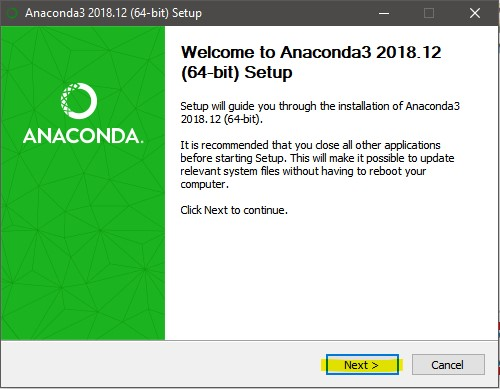
\includegraphics[height=3cm]{figures/1/1174066/gambar/install1.jpg}
  \caption{Tampilan Instalasi 1}
\end{figure}

  \item Baca license agreement lalu tekan 'I Agree'
\begin{figure}[!htbp]
  \centering
  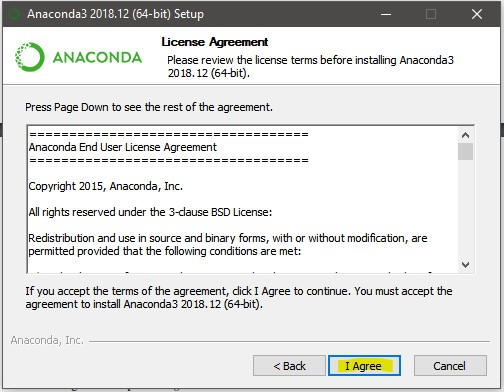
\includegraphics[height=3cm]{figures/1/1174066/gambar/install2.jpg}
  \caption{Tampilan Instalasi 2}
\end{figure}

  \item Setelah itu pilih mau diinstall pada user yang sedang anda pakai atau kesemua user, direkomendasikan untuk memilih just me yaitu hanya user yang sedang dipakai saja
\begin{figure}[!htbp]
  \centering
  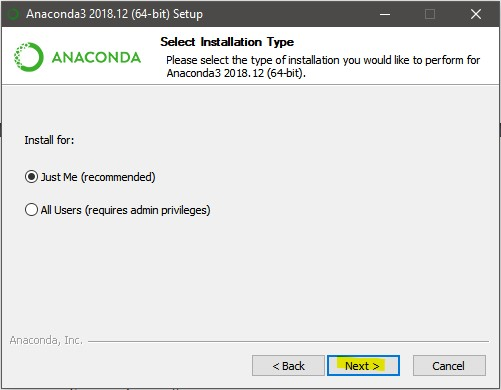
\includegraphics[height=3cm]{figures/1/1174066/gambar/install3.jpg}
  \caption{Tampilan Instalasi 3}
\end{figure}

  \item Catat tempat dimana anda akan menginstall anaconda, lalu tekan 'Next'
\begin{figure}[!htbp]
  \centering
  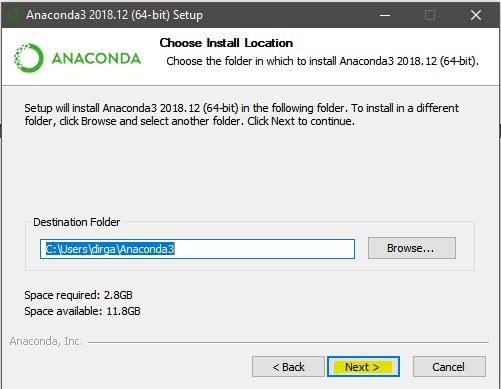
\includegraphics[height=3cm]{figures/1/1174066/gambar/install4.jpg}
  \caption{Tampilan Instalasi 4}
\end{figure}

  \item Setelah itu anda diberi pilihan, direkomendasikan untuk tidak mengubah pilihan tersebut, lalu tekan 'Install'
\begin{figure}[!htbp]
  \centering
  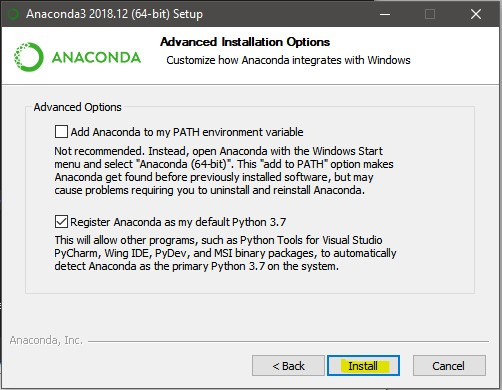
\includegraphics[height=3cm]{figures/1/1174066/gambar/install5.jpg}
  \caption{Tampilan Instalasi 5}
\end{figure}

  \item Tunggu sampai instalasi selesai
\begin{figure}[!htbp]
  \centering
  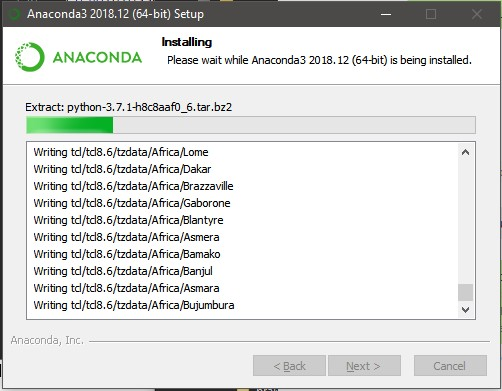
\includegraphics[height=3cm]{figures/1/1174066/gambar/install6.jpg}
  \caption{Tampilan Instalasi 6}
\end{figure}

  \item Setelah selesai tekan 'Next'
\begin{figure}[!htbp]
  \centering
  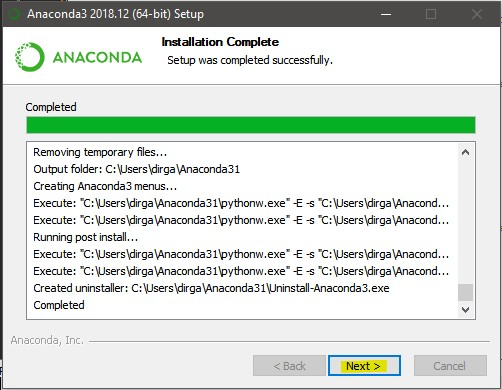
\includegraphics[height=3cm]{figures/1/1174066/gambar/install7.jpg}
  \caption{Tampilan Instalasi 7}
\end{figure}

  \item Setelah itu ada opsi untuk memilih untuk meinstall visual studio code, jika anda berminat klik 'Install VSCode' jika tidak tekan 'Skip'
\begin{figure}[!htbp]
  \centering
  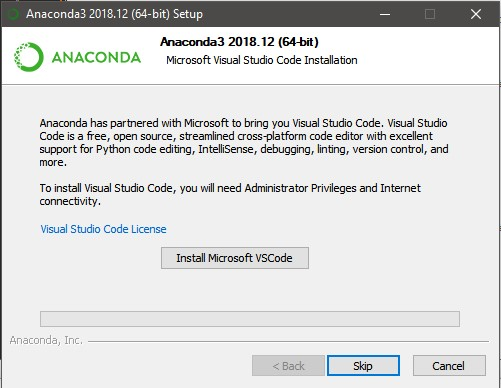
\includegraphics[height=3cm]{figures/1/1174066/gambar/install8.jpg}
  \caption{Tampilan Instalasi 8}
\end{figure}

  \item Tekan 'Finish' untuk menyelesaikan instalasi
\begin{figure}[!htbp]
  \centering
  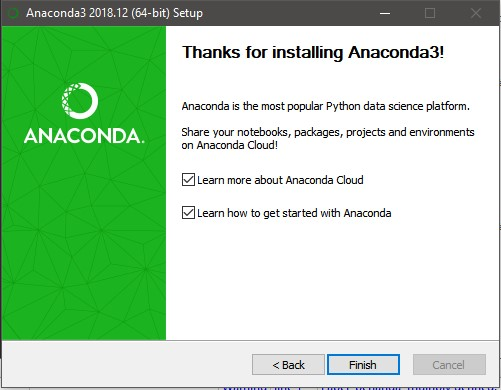
\includegraphics[height=3cm]{figures/1/1174066/gambar/install9.jpg}
  \caption{Tampilan Instalasi 9}
\end{figure}

\end{enumerate}

\subsection{Cara menggunakan Spyder pada Anaconda}
Pertama buka aplikasi Anaconda sampai muncul seperti ini
\begin{figure}[!htbp]
  \centering
  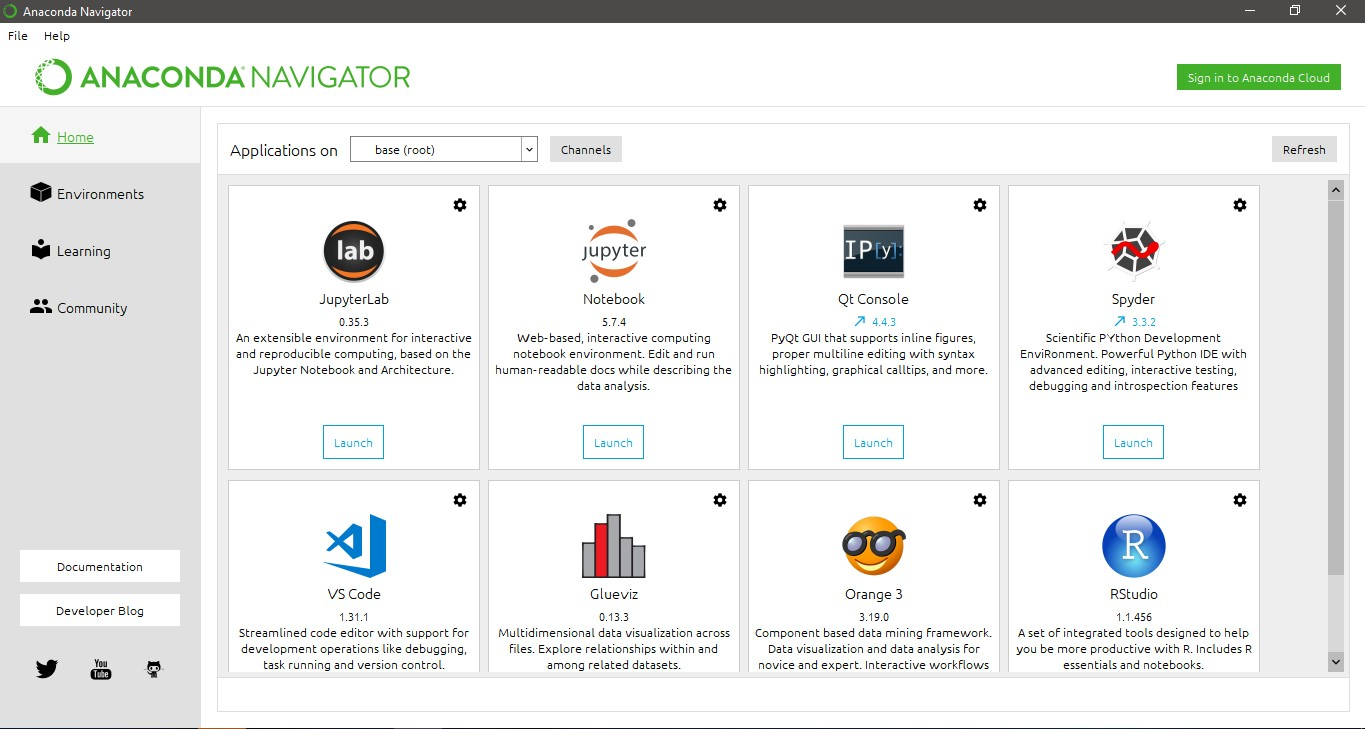
\includegraphics[height=3cm]{figures/1/1174066/gambar/gambaranaconda.jpg}
  \caption{Tampilan awal Anaconda}
\end{figure}

Setelah itu tekan Launch dibawah logo Spyder
Tunggu sampai muncul seperti ini
\begin{figure}[!htbp]
  \centering
  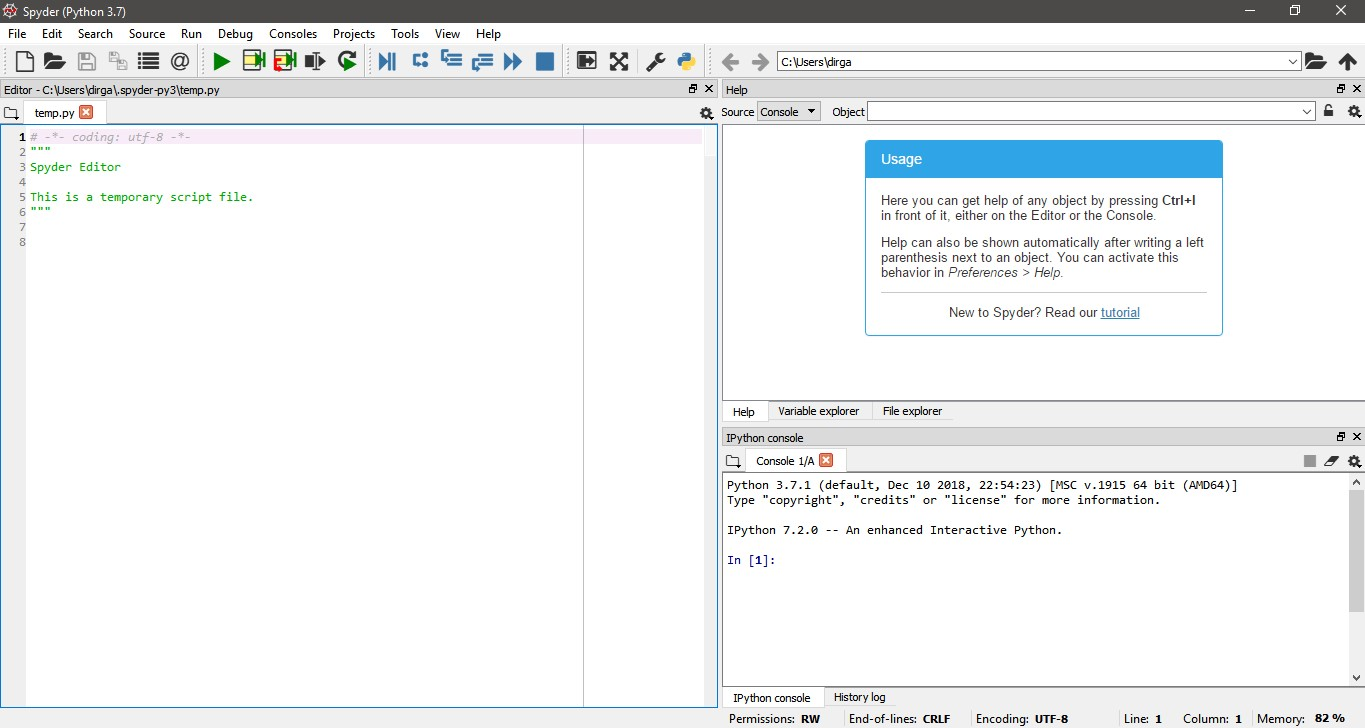
\includegraphics[height=3cm]{figures/1/1174066/gambar/gambarspider.jpg}
  \caption{Tampilan spider}
\end{figure}

\subsection{Membuat Hello World di Spyder}
Setelah membuka spyder seperti gambar di section sebelumnya tekan menu File lalu klik New File atau bisa menggunakan kombinasi tombol Ctrl + N sampai muncul seperti ini

\begin{figure}[!htbp]
  \centering
  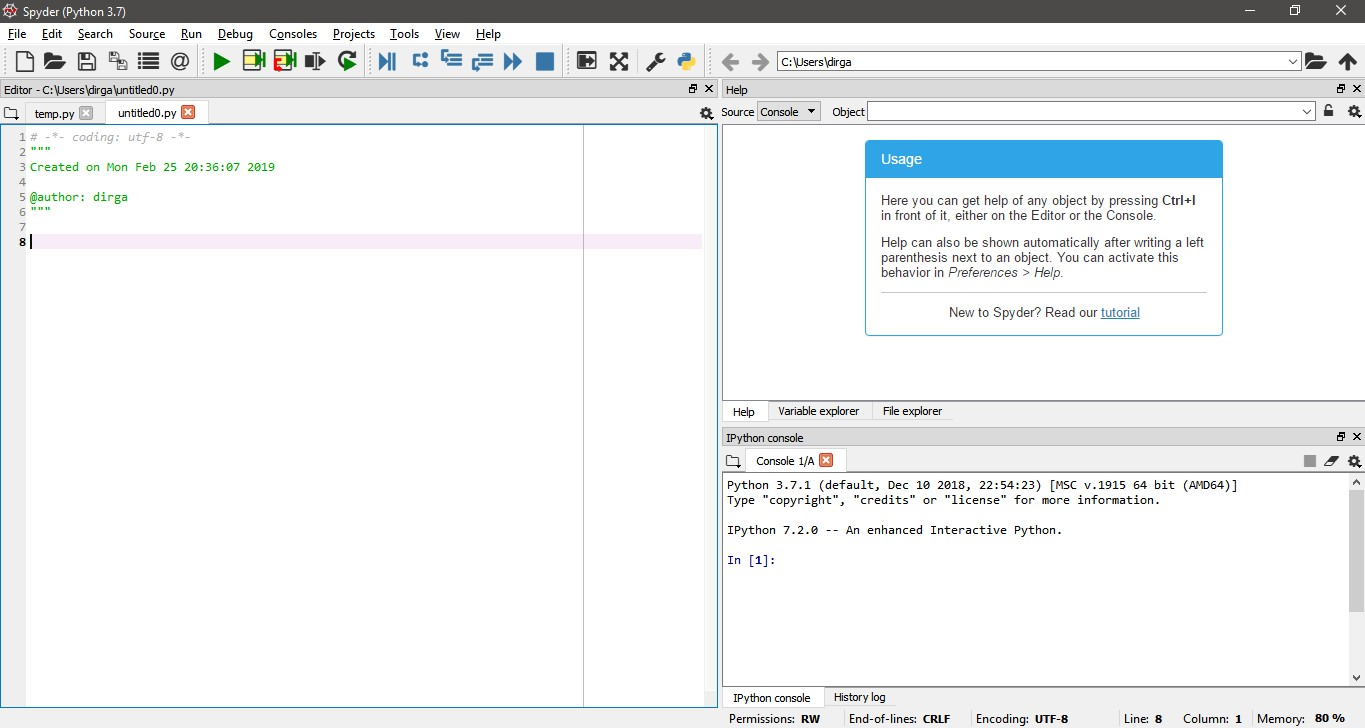
\includegraphics[height=3cm]{figures/1/1174066/gambar/gambarnewfile.jpg}
  \caption{Tampilan new file pada spider}
\end{figure}

Karena kita menggunakan Python3.7 maka kita menggunakan funsi print() untuk memunculkan teks Hello World yang akan kita buat, tuliskan print("Hello World") pada teks editor di Spyder

\begin{figure}[!htbp]
  \centering
  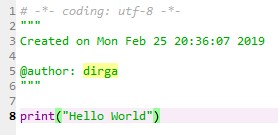
\includegraphics[height=3cm]{figures/1/1174066/gambar/gambarprint.jpg}
  \caption{print("Hello World")}
\end{figure}

setelah itu tekan tombol play berwarna hijau diatas, karena kita belum save file yang kita buat maka akan muncul dialog simpan file, pilih tempat dan nama file yang akan disimpan contohnya helloworld.py

\begin{figure}[!htbp]
  \centering
  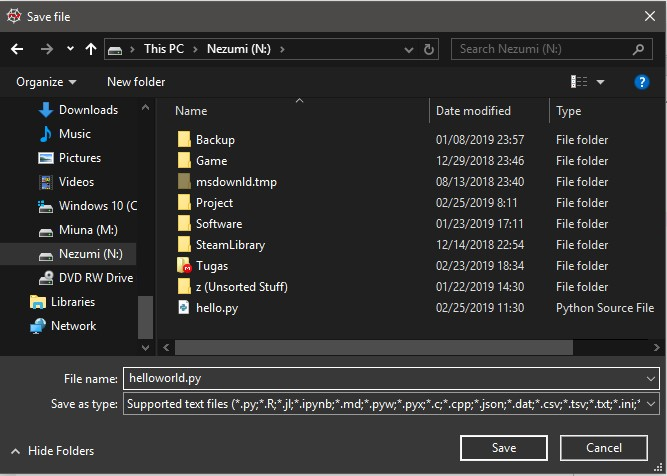
\includegraphics[height=3cm]{figures/1/1174066/gambar/helloworld.jpg}
  \caption{Dialog simpan file}
\end{figure}

setelah itu tekan run maka hasil dari program yang kita buat tadi ada dibagian console yang berada di pinggir kanan bawah

\begin{figure}[!htbp]
  \centering
  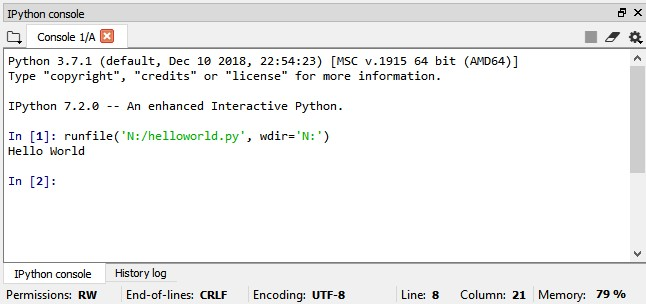
\includegraphics[height=3cm]{figures/1/1174066/gambar/hasil.jpg}
  \caption{Hasil Program}
\end{figure}


%PRAKTEK
%\chapter{Judul Bagian Pertama}
%\section{Arjun Yuda Firwanda}
\subsection{Soal 1}
Isi jawaban soal ke-1

Kalau mau dibikin paragrap \textbf{cukup enter aja}, tidak usah pakai \verb|par| dsb

%\subsection{Soal 2}
%Isi jawaban soal ke-2

%\subsection{Soal 3}
%Isi jawaban soal ke-3

\section{Dwi Yulianingsih}
\subsection{Soal 1}
Isi jawaban soal ke-1

Kalau mau dibikin paragrap \textbf{cukup enter aja}, tidak usah pakai \verb|par| dsb

%\subsection{Soal 2}
%Isi jawaban soal ke-2

%\subsection{Soal 3}
%Isi jawaban soal ke-3

\section{Harun Ar-Rasyid}
\subsection{Soal 1}
Isi jawaban soal ke-1

Kalau mau dibikin paragrap \textbf{cukup enter aja}, tidak usah pakai \verb|par| dsb

%\subsection{Soal 2}
%Isi jawaban soal ke-2

%\subsection{Soal 3}
%Isi jawaban soal ke-3

\section{Sri Rahayu}
\subsection{Soal 1}
Isi jawaban soal ke-1

Kalau mau dibikin paragrap \textbf{cukup enter aja}, tidak usah pakai \verb|par| dsb

%\subsection{Soal 2}
%Isi jawaban soal ke-2

%\subsection{Soal 3}
%Isi jawaban soal ke-3

\section{Doli Jonviter}
\subsection{Soal 1}
Isi jawaban soal ke-1

Kalau mau dibikin paragrap \textbf{cukup enter aja}, tidak usah pakai \verb|par| dsb

%\subsection{Soal 2}
%Isi jawaban soal ke-2

%\subsection{Soal 3}
%Isi jawaban soal ke-3

\section{Rahmatul Ridha}
\subsection{Soal 1}
Isi jawaban soal ke-1

Kalau mau dibikin paragrap \textbf{cukup enter aja}, tidak usah pakai \verb|par| dsb

%\subsection{Soal 2}
%Isi jawaban soal ke-2

%\subsection{Soal 3}
%Isi jawaban soal ke-3

\section{Tomy Prawoto}
\subsection{Soal 1}
Isi jawaban soal ke-1

Kalau mau dibikin paragrap \textbf{cukup enter aja}, tidak usah pakai \verb|par| dsb

%\subsection{Soal 2}
%Isi jawaban soal ke-2

%\subsection{Soal 3}
%Isi jawaban soal ke-3


%TEORI
\chapter{Pemograman Dasar}
\section{D. Irga B. Naufal Fakhri}
\subsection{Teori}
\begin{enumerate}
\item Jenis-jenis variabel pada python dan cara penggunaannya:

\begin{enumerate}
\item Boolean
\lstinputlisting[caption=Contoh kode variable Boolean., firstline=8, lastline=10]{src/2/1174066/1174066.py}

\item String
\lstinputlisting[caption=Contoh kode variable String., firstline=12, lastline=14]{src/2/1174066/1174066.py}

\item Integer
\lstinputlisting[caption=Contoh kode variable Integer., firstline=16, lastline=18]{src/2/1174066/1174066.py}

\item Float
\lstinputlisting[caption=Contoh kode variable Float., firstline=20, lastline=22]{src/2/1174066/1174066.py}

\item Hexadecimal
\lstinputlisting[caption=Contoh kode variable Hexadecimal., firstline=24, lastline=26]{src/2/1174066/1174066.py}

\item Complex
\lstinputlisting[caption=Contoh kode variable Complex., firstline=28, lastline=30]{src/2/1174066/1174066.py}

\item List
\lstinputlisting[caption=Contoh kode variable List., firstline=32, lastline=35]{src/2/1174066/1174066.py}

\item Tuple
\lstinputlisting[caption=Contoh kode variable Tuple., firstline=37, lastline=40]{src/2/1174066/1174066.py}

\item Set
\lstinputlisting[caption=Contoh kode variable Set., firstline=42, lastline=44]{src/2/1174066/1174066.py}

\item Dictionary
\lstinputlisting[caption=Contoh kode variable Dictionary., firstline=46, lastline=49]{src/2/1174066/1174066.py}

\end{enumerate}

\item Permintaan Input dari user dan Outputnya
\lstinputlisting[caption=Contoh kode input dan outputnya., firstline=51, lastline=53]{src/2/1174066/1174066.py}

\item Operator dasar aritmatika dan perubahan tipe data variable

Operator dasar aritmatika
\begin{enumerate}
\item Perjumlahan (+)
Operator ini berfungsi untuk melakukan operasi perjumlahan.
\lstinputlisting[caption=Contoh kode operasi pertambahan., firstline=51, lastline=60]{src/2/1174066/1174066.py}
\item Pengurangan (-)
Operator ini berfungsi untuk melakukan operasi pengurangan.
\lstinputlisting[caption=Contoh kode operasi pengurangan., firstline=62, lastline=66]{src/2/1174066/1174066.py}
\item Perkalian (*)
Operator ini dipergunakan untuk melakukan operasi perkalian.
\lstinputlisting[caption=Contoh kode operasi perkalian., firstline=68, lastline=72]{src/2/1174066/1174066.py}
\item Pembagian (/)
Operator ini dipergunakan untuk melakukan operasi pembagian.
\lstinputlisting[caption=Contoh kode operasi pembagian., firstline=74, lastline=78]{src/2/1174066/1174066.py}
\item Modulus (%)
Operator ini dipergunakan untuk melakukan operasi modulus.
\lstinputlisting[caption=Contoh kode operasi modulus., firstline=80, lastline=84]{src/2/1174066/1174066.py}
\item Perpangkatan (**)
Operator ini dipergunakan untuk melakukan operasi perpangkatan.
\lstinputlisting[caption=Contoh kode operasi perpangkatan., firstline=86, lastline=90]{src/2/1174066/1174066.py}
\item Pembulatan Kebawah Pada Hasil Pembagian (//)
Operator ini dipergunakan untuk melakukan operasi pembulatan hasil bagi.
\lstinputlisting[caption=Contoh kode operasi pembulatan hasil pembagian kebawah., firstline=92, lastline=96]{src/2/1174066/1174066.py}
\end{enumerate}

Perubahan tipe data variable
\begin{enumerate}
\item String menjadi Integer
\lstinputlisting[caption=Contoh kode variable string menjadi integer., firstline=99, lastline=102]{src/2/1174066/1174066.py}
\item Integer menjadi String
\lstinputlisting[caption=Contoh kode variable integer menjadi string., firstline=104, lastline=107]{src/2/1174066/1174066.py}
\end{enumerate}


\item Sintak perulangan (looping), jenis-jenisnya, dan penggunaannya.
\begin{enumerate}
\item While Loop
While Loop adalah perulangan yang mengeksekusi statement terus menerus selama kondisi bernilai True.
\lstinputlisting[caption=Contoh kode penggunaan while loop., firstline=111, lastline=115]{src/2/1174066/1174066.py}

\item For Loop
For Loop  adalah pengulangan berdasarkan kondisi yang telah ditentukan biasanya kondisi pertambahan seperti 1 sampai 5
\lstinputlisting[caption=Contoh kode penggunaan for loop., firstline=117, lastline=120]{src/2/1174066/1174066.py}

\item Nested Loop
Nested Loop merupakan pengulangan yang ada di dalam pengulangan
\lstinputlisting[caption=Contoh kode penggunaan nested loop., firstline=122, lastline=129]{src/2/1174066/1174066.py}

\end{enumerate}

\item Sintak kondisi dan penggunaannya.
\begin{enumerate}
\item If
Kondisi ini digunakan untuk mengecek apabila kondisi tersebut dipenuhi akan mengeksekusi kode didalamnya.
\lstinputlisting[caption=Contoh kode penggunaan if., firstline=132, lastline=136]{src/2/1174066/1174066.py}

\item If Else
Kondisi ini digunakan untuk mengecek apabila kondisi tersebut dipenuhi akan mengeksekusi kode didalamnya dan didalamnya memiliki dua kondisi.
\lstinputlisting[caption=Contoh kode penggunaan if else., firstline=138, lastline=143]{src/2/1174066/1174066.py}

\item Elif
Kondisi ini digunakan untuk mengecek apabila kondisi tersebut dipenuhi akan mengeksekusi kode didalamnya dan didalamnya memiliki dua kondisi atau lebih.
\lstinputlisting[caption=Contoh kode penggunaan elif., firstline=145, lastline=152]{src/2/1174066/1174066.py}

\item Kondisi di dalam kondisi
Kondisi ini digunakan saat kondisi memerlukan kondisi lagi didalamnya
\lstinputlisting[caption=Contoh kode penggunaan kondisi di dalam kondisi., firstline=155, lastline=165]{src/2/1174066/1174066.py}

\end{enumerate}

\item Jenis-jenis error pada python dan cara mengatasinya.
\begin{itemize}
\item Syntax Errors
Syntax Errors adalah kesalahan pada penulisan syntax atau kode. Solusinya adalah memperbaiki penulisan syntax atau kode

\item Zero Division Error
ZeroDivisonError adalah exceptions yang terjadi saat eksekusi program menghasilkan perhitungan matematika pembagian dengan angka nol (0). Solusinya adalah tidak membagi suatu yang hasilnya nol.

\item Name Error
NameError adalah exception saat kode melakukan eksekusi terhadap local name atau global name yang tidak terdefinisi atau tidak ada. Solusinya adalah memastikan variabel atau function yang akan dipanggil ada didalam program atau tidak salah mengetikannya.

\item Type Error
TypeError adalah exception saat melakukan eksekusi terhadap suatu operasi atau fungsi dengan type object yang tidak sesuai. Solusinya adalah mengkoversi varibelnya sesuai dengan tipe data sesuai dengan yang akan digunakan.

\end{itemize}

\item Cara pemakaian Try Except.
\lstinputlisting[caption=Contoh kode penggunaan try except., firstline=168, lastline=174]{src/2/1174066/1174066.py}

\end{enumerate}
%PRAKTEK
\chapter{Praktek Pemograman Dasar}
\section{Arjun Yuda Firwanda}
\subsection{Soal 1}
Isi jawaban soal ke-1

Kalau mau dibikin paragrap \textbf{cukup enter aja}, tidak usah pakai \verb|par| dsb

%\subsection{Soal 2}
%Isi jawaban soal ke-2

%\subsection{Soal 3}
%Isi jawaban soal ke-3

\section{Dwi Yulianingsih}
\subsection{Soal 1}
Isi jawaban soal ke-1

Kalau mau dibikin paragrap \textbf{cukup enter aja}, tidak usah pakai \verb|par| dsb

%\subsection{Soal 2}
%Isi jawaban soal ke-2

%\subsection{Soal 3}
%Isi jawaban soal ke-3

\section{Harun Ar-Rasyid}
\subsection{Soal 1}
Isi jawaban soal ke-1

Kalau mau dibikin paragrap \textbf{cukup enter aja}, tidak usah pakai \verb|par| dsb

%\subsection{Soal 2}
%Isi jawaban soal ke-2

%\subsection{Soal 3}
%Isi jawaban soal ke-3

\section{Sri Rahayu}
\subsection{Soal 1}
Isi jawaban soal ke-1

Kalau mau dibikin paragrap \textbf{cukup enter aja}, tidak usah pakai \verb|par| dsb

%\subsection{Soal 2}
%Isi jawaban soal ke-2

%\subsection{Soal 3}
%Isi jawaban soal ke-3

\section{Doli Jonviter}
\subsection{Soal 1}
Isi jawaban soal ke-1

Kalau mau dibikin paragrap \textbf{cukup enter aja}, tidak usah pakai \verb|par| dsb

%\subsection{Soal 2}
%Isi jawaban soal ke-2

%\subsection{Soal 3}
%Isi jawaban soal ke-3

\section{Rahmatul Ridha}
\subsection{Soal 1}
Isi jawaban soal ke-1

Kalau mau dibikin paragrap \textbf{cukup enter aja}, tidak usah pakai \verb|par| dsb

%\subsection{Soal 2}
%Isi jawaban soal ke-2

%\subsection{Soal 3}
%Isi jawaban soal ke-3

\section{Tomy Prawoto}
\subsection{Soal 1}
Isi jawaban soal ke-1

Kalau mau dibikin paragrap \textbf{cukup enter aja}, tidak usah pakai \verb|par| dsb

%\subsection{Soal 2}
%Isi jawaban soal ke-2

%\subsection{Soal 3}
%Isi jawaban soal ke-3


%TEORI
\chapter{Fungsi dan Kelas}
\section{D. Irga B. Naufal Fakhri}
\subsection{Pemahaman Teori}
\begin{enumerate}
\item Fungsi

Fungsi adalah blok blok kode yang teroorganisir yang dapat digunakan kembali didalam program yang digunakan untuk melakukan suatu perintah yang telah diberikan.
untuk membuat fungsi kita harus menggunakan def kemudian nama fungsinya dan (variable)nya diakhiri oleh tanda :
\lstinputlisting[caption=Contoh kode fungsi inputan ke fungsi., firstline=296, lastline=301]{src/3/1174066/1174066.py}
Fungsi juga berguna untuk melemparkan variable contohnya
\lstinputlisting[caption=Contoh kode fungsi outputan ke fungsi., firstline=303, lastline=308]{src/3/1174066/1174066.py}

\item Paket(Package) atau Libary

Paket atau yang biasa disebut dengan library adalah kumpulan kode-kode fungsi atau method pada python yang dapat dipanggil kedalam program python yang kita buat. Package berada di file terpisah dari main program
cara memanggil package: Pastikan file package ada didalam folder yang sama lalu ditambah import dengan nama filenya tanpa extensi (.py)
\lstinputlisting[caption=Contoh import package atau library., firstline=311, lastline=314]{src/3/1174066/1174066.py}

\item Kelas (Class), Objek (Object), Atribut (Attribute), dan Method

Kelas(Class) adalah sebuah blueprint(cetakan) dari sebuah objek.
Objek(Object) adalah hasil cetakan dari sebuah kelas(class).
Atribut(Attribute) adalah nilai data yang ada didalam sebuah object.
Method adalah sesuatu yang bisa dilakukan oleh object.

\lstinputlisting[caption=Contoh import package atau library., firstline=316, lastline=328]{src/3/1174066/1174066.py}

\item Cara memanggil library dari instansiasi

Cara memanggilnya:
\begin{itemize}
	\item Pertama kita import filenya
	\item kemudian buat variablenya jika menggunakan variable untuk menampung data
	\item Kemudian panggil nama classnya(file) dan panggil fungsinya
	\item Kemudian menggunakan perintah print untuk menampilkan data
\end{itemize}
\lstinputlisting[caption=Contoh package atau library., firstline=6, lastline=9]{src/3/1174066/fungsi_1174066.py} 
\lstinputlisting[caption=Contoh import package atau library., firstline=331, lastline=336]{src/3/1174066/1174066.py}

\item  Contoh pemakaian paket dengan perintah from kalkulator import Penambahan 

Pemakaian package(paket) dengan perintah from namafilenya import berfungsi untuk memanggil fungsi dari nama filenya
\lstinputlisting[caption=Contoh import package atau library., firstline=339, lastline=344]{src/3/1174066/1174066.py}

\item Jelaskan dengan contoh kode, pemakaian paket fungsi didalam folder

Jika file paket ada didalam folder maka kita harus menambahkan lokasi filenya ada didalam folder apa dengan cara menggunakan namafolder.namafile
\lstinputlisting[caption=Contoh import package atau library didalam folder., firstline=346, lastline=351]{src/3/1174066/1174066.py}

\item Jelaskan dengan contoh kode, pemakaian paket fungsi didalam folder

Jika file paket ada didalam folder maka kita harus menambahkan lokasi filenya ada didalam folder apa dengan cara menggunakan namafolder.namafile
\lstinputlisting[caption=Contoh import package atau library didalam folder., firstline=346, lastline=351]{src/3/1174066/1174066.py}
\end{enumerate}
%PRAKTEK
\chapter{Praktek Fungsi dan Kelas}
\section{D. Irga B. Naufal Fakhri}
\subsection{Keterampilan Pemograman}
\begin{enumerate}
\item Jawaban nomor 1
\lstinputlisting[firstline=355, lastline=373]{src/3/1174066/1174066.py}

\item Jawaban nomor 2
\lstinputlisting[firstline=377, lastline=384]{src/3/1174066/1174066.py}

\item Jawaban nomor 3
\lstinputlisting[firstline=386, lastline=394]{src/3/1174066/1174066.py}

\item Jawaban nomor 4
\lstinputlisting[firstline=396, lastline=400]{src/3/1174066/1174066.py}

\item Jawaban nomor 5
\lstinputlisting[firstline=402, lastline=405]{src/3/1174066/1174066.py}

\item Jawaban nomor 6
\lstinputlisting[firstline=410, lastline=418]{src/3/1174066/1174066.py}

\item Jawaban nomor 7
\lstinputlisting[firstline=420, lastline=428]{src/3/1174066/1174066.py}

\item Jawaban nomor 8
\lstinputlisting[firstline=431, lastline=439]{src/3/1174066/1174066.py}

\item Jawaban nomor 9
\lstinputlisting[firstline=441, lastline=448]{src/3/1174066/1174066.py}

\item Jawaban nomor 10
\lstinputlisting[firstline=451, lastline=468]{src/3/1174066/1174066.py}

\item Jawaban nomor 11
\lstinputlisting[firstline=8, lastline=20]{src/3/1174066/main_1174066.py}

\item Jawaban nomor 12
\lstinputlisting[firstline=23, lastline=37]{src/3/1174066/main_1174066.py}
\end{enumerate}

\subsection{Ketrampilan Penanganan Error}
\begin{itemize}
\item Syntax Errors

Syntax Errors adalah kesalahan pada penulisan syntax atau kode. Solusinya adalah memperbaiki penulisan syntax atau kode

\item Zero Division Error

ZeroDivisonError adalah exceptions yang terjadi saat eksekusi program menghasilkan perhitungan matematika pembagian dengan angka nol (0). Solusinya adalah tidak membagi suatu yang hasilnya nol.

\item Name Error

NameError adalah exception saat kode melakukan eksekusi terhadap local name atau global name yang tidak terdefinisi atau tidak ada. Solusinya adalah memastikan variabel atau function yang akan dipanggil ada didalam program atau tidak salah mengetikannya.

\item Type Error

TypeError adalah exception saat melakukan eksekusi terhadap suatu operasi atau fungsi dengan type object yang tidak sesuai. Solusinya adalah mengkoversi varibelnya sesuai dengan tipe data sesuai dengan yang akan digunakan.
\end{itemize}
\lstinputlisting[firstline=23, lastline=37]{src/3/1174066/main_1174066.py}

%TEORI
\chapter{Library CSV dan Pandas}
\section{D. Irga B. Naufal Fakhri}
\subsection{Pemahaman Teori}
\begin{enumerate}
\item CSV

CSV (Comma Separated Values file) adalah sebuah tipe file text biasa yang memiliki penataan khusus yang biasanya berfungsi untuk mengelola data. sesuai dengan namanya file csv memisahkan setiap data menggunakan koma (,).

Format data CSV pertama kali digunakan pada tahun 1978 pada complier FORTRAN 77, kemudian nama CSV baru muncul dan mulai digunakan pada tahun 1983 

Contoh data pada csv:
\lstinputlisting[firstline=0, lastline=2]{src/4/1174066/Teori/1174066.csv}

\item Aplikasi yang bisa menciptakan CSV

Semua aplikasi teks editor seperti notepad++, vscode, sublime ataupun notepad dapat menciptakan CSV termasuk aplikasi spreadsheet seperti Microsoft Excel, Libre Office 

\item Jelaskan bagaimana cara menulis dan membaca file csv di Excel atau spreadsheet

\begin{itemize}
	\item Buka Microsoft Excel 2019-nya lalu buat dokumen baru
	\item Isikan data sesuai dengan kebutuhan, yang paling atas akan menjadi header dari file csv
	\item Setelah memasukkan data, klik file lalu klik Save As
	\item Pilih Browse dan pilih tempat menyimpannya akan dimana
	\item Masukkan nama file pada File Name
	\item Lalu pada Save As Type pilih CSV (comma delimited) (*.csv)
	\item Maka hasil file akan seperti ini
	\lstinputlisting[firstline=0, lastline=2]{src/4/1174066/Teori/1174066.csv}
\end{itemize}

\item Jelaskan sejarah library csv

Module csv mengimplementasikan kelas untuk membaca dan menulis data kedalam format CSV. Hal ini memungkinkan programmer untuk "tulis data ini dalam format yang disukai oleh Excel," atau "baca data dari file yang dihasilkan oleh Excel," tanpa mengetahui detail yang tepat dari format CSV yang digunakan oleh Excel. Pemrogram juga dapat menggambarkan format CSV yang dipahami oleh aplikasi lain atau menentukan format CSV tujuan khusus untuk mereka sendiri.

\item Jelaskan sejarah library pandas

pandas adalah sebuah library open source dan berlisensi BSD yang menyediakan performa yang tinggi, mudah digunakan struktur data dan data analisis untuk python.

\item Jelaskan fungsi-fungsi yang terdapat di library csv
\begin{itemize}
	\item csv.reader
	
	Berfungsi untuk membaca dan mengembalikan data kedalam variable dari file csv.
	Fungsi reader dirancang untuk mengambil data pada setiap baris didalam file dan membuat daftar semua kolom. Kemudian, tinggal dipilih kolom mana yang diinginkan untuk data variabel.
	\lstinputlisting[firstline=9, lastline=22]{src/4/1174066/Teori/1174066_csv.py}
	
	\item csv.writer
	
	Berfungsi untuk menuliskan data dari variable kedalam file csv.
	Fungsi writer akan membuat objek yang cocok untuk menulis. Untuk mengulang data yang ada di atas baris, gunakan fungsi writerow.
	\lstinputlisting[firstline=38, lastline=45]{src/4/1174066/Teori/1174066_csv.py}
	
	\item csv.register\textunderscore dialect
	
	Mendaftarkan dialect pada csv
	\item csv.unregister\textunderscore dialect
	
	Menghapus dialect yang diasosiasi dengan nama dari registry dialect
	
	\item csv.list\textunderscore dialects
	
	Mengembalikan dialect yang diasosiasi dengan nama
	
	\item csv.field\textunderscore size\textunderscore limit
	
	Mengembalikan ukuran field maksimum yang diizinkan oleh parser.
	
	\item csv.DictReader
	
	Berfungsi untuk membaca dan mengembalikan data kedalam variable dictionary dari file csv.
	\lstinputlisting[firstline=24, lastline=36]{src/4/1174066/Teori/1174066_csv.py}
	
\end{itemize}

\item Jelaskan fungsi-fungsi yang terdapat di library pandas
\begin{itemize}
	\item pandas.read\textunderscore csv
	
	Berfungsi untuk membaca dan mengembalikan data kedalam format DataFrame dari file csv.
	\lstinputlisting[firstline=9, lastline=13]{src/4/1174066/Teori/1174066_pandas.py}
	
	\item to\textunderscore dict
	
	Berfungsi untuk membaca dan mengembalikan data kedalam format dictionary dari file csv.
	\lstinputlisting[firstline=15, lastline=19]{src/4/1174066/Teori/1174066_pandas.py}
	
	\item to\textunderscore csv
	
	Berfungsi untuk mengedit data didalam csv dan menulisnya kedalam file csv
	\lstinputlisting[firstline=42, lastline=49]{src/4/1174066/Teori/1174066_pandas.py}
\end{itemize}
\end{enumerate}

%%%%%%%%%%%%%%%%%%%%%%%%%%%%%%%%%%%%%%%%%%%%%%%%%%%%%%%%%%%%%%%%%%%%%%%%%%%%%%%%%%%%%%%%%%%%%%%%%%%%%%%%%%%%%%%%%%%%%%%%%%
\section{Fanny Shafira Damayanti | 1174069}
\subsection{Pemahaman Teori}
\begin{enumerate}
\item Fungsi CSV, sejarah dan contoh

CSV (comma separated value) digunakan pada tahun 1983 merupakan suatu tipe file yang digunakan untuk pengolahan informasi yang dihasilkan spreadsheet yang di proses melalui mesin analitik. CSV juga digunakan sebagai file yang agnostik karena bisa digunakan olej berbagai database untuk backup data.

Contoh :

\lstinputlisting[firstline=7, lastline=28]{src/4/1174069/Teori/1174069_csvteori.py}

\item Aplikasi untuk membuat file CSV

\begin{itemize}
\item Microsoft Excel
\item Spyder
\item Apple Number
\item LibrareOffice
\item Apple Office Calc
\item Apache Open Office Calc

\end{itemize}

\item Cara menulis dan membaca file .csv di Excel atau Spreadsheet

Cara menulis :

Buka Ms. Excel, lalu buat file nya, ketika akan di save ganti jenis filenya menjadi .csv
\begin{itemize}
\item Download Template CSV.
\item Buka file spreadsheet Anda di Excel. 
\item Buat dokumen baru di Excel.
\item Tambahkan judul kolom, lalu ketikkan informasi dalam kolom tersebut
\item Klik File , dan pilih Save As 
\item Masukkan nama file, lalu pilih CSV (Comma delimited) (* csv) dari drop-down Save as type .
\end{itemize}


Cara membaca :

\begin{itemize}
\item Buka Microsoft Excel.
\item Mulai / buka spreadsheet 
\item Pilih tab Data 
\item Pilih opsi Dari Teks. (Jika opsi berwarna abu-abu, Anda \item mungkin perlu membuka spreadsheet / workbook baru).
\item Temukan dan pilih file .csv yang telah Anda unduh dari \item Kotive. Klik pada file dan kemudian klik Impor.
\item Panduan impor Teks akan terbuka. Pastikan opsi Dibatasi  dipilih. Klik tombol Berikutnya.
\item Pilih Koma di bawah Pembatas. Kualifikasi Teks harus menunjukkan “(tanda kutip ganda). Klik tombol Selesai.
Anda mungkin ditanya Di mana Anda ingin meletakkan data? Klik pada sel kiri atas. Klik tombol OK.
\item Excel menampilkan data di buku kerja Anda
\end{itemize}



\item Sejarah Libary CSV
Inisiatif standardisasi utama - mentransformasikan "definisi fuzzy de facto" menjadi definisi yang lebih tepat dan de jure - adalah pada tahun 2005, dengan RFC4180, mendefinisikan CSV sebagai Tipe Konten MIME. Kemudian, pada 2013, beberapa kekurangan RFC4180 ditangani oleh rekomendasi W3C.

Pada 2014 IETF menerbitkan RFC7111 yang menjelaskan aplikasi fragmen URI pada dokumen CSV. RFC7111 menentukan bagaimana rentang baris, kolom, dan sel dapat dipilih dari dokumen CSV menggunakan indeks posisi.

Pada 2015 W3C, dalam upaya untuk meningkatkan CSV dengan semantik formal, mempublikasikan draft rekomendasi pertama untuk standar metadata CSV, yang dimulai sebagai rekomendasi pada bulan Desember tahun yang sama.

\item Sejarah Libarary Pandas

Pandas muncul ketika ada bahasa pemrograman R dan Matlab.
Pengembang Wes McKinney mulai mengerjakan pandas pada 2008 ketika di AQR Capital Management karena kebutuhan akan alat kinerja tinggi yang fleksibel untuk melakukan analisis kuantitatif pada data keuangan. Sebelum meninggalkan AQR, dia bisa meyakinkan manajemen untuk mengizinkannya membuka sumber perpustakaan.

Pegawai AQR lainnya, Chang She, bergabung dengan upaya ini pada 2012 sebagai kontributor utama kedua ke perpustakaan.

Pada 2015, panda menandatangani sebagai proyek NumFOCUS yang disponsori secara fiskal, sebuah badan amal nirlaba 501 (c) (3) di Amerika Serikat.

\item Fungsi yang terdapat pada Library CSV

\begin{itemize}
\item csv.reader berfungsi untuk membaca modul csv.
\item csv.writer berfungsi untuk menulis modul csv.
\item csv.writerows berfungsi untuk menambahkan baris baru.
\end{itemize}

\item Fungsi yag terdapat pada Libarary Pandas

Dengan panda kita dapat dengan mudah merubah data (CSV, excel, JSON atau SQL) menjadi sebuah object data yang terdiri dari baris dan kolom yang disebut dengan DataFrame.
Fitur :

\begin{itemize}

\item DataFrame Object untuk manipulasi data dengan pengindeksan terintegrasi.
\item Alat untuk membaca dan menulis data antara struktur data dalam memori dan berbagai format file.
\item Penyelarasan data dan penanganan terpadu pada kehilangan data.
\item Membentuk kembali dan memutar set data.
\item Seleksi berbasis label, pengindeksan fantastis, dan melakukan subset kumpulan data besar.
\item Penyisipan dan penghapusan kolom struktur data.
\item Memungkinkan operasi split-apply-combine pada Data set.
\item Menghubugkan dan menggabungkan Data set.
\item Pengindeksan hierarki untuk bekerja dengan data dimensi tinggi dalam struktur data dimensi rendah.
\item Fungsionalitas seri waktu: Pembuatan rentang tanggal dan konversi frekuensi.
\item Menyediakan penyaringan data (sorting dan filtering).
\end{itemize}


\end{enumerate}

%%%%%%%%%%%%%%%%%%%%%%%%%%%%%%%%%%%%%%%%%%%%%%%%%%%%%%%%%%%%%%%%%%%%%%%%%%%%%%%%%%%%%%%%%%%%%%%%%%%%%%%%%%%%%%%%%%%%
\section{Aulyardha Anindita | 1174054}

\subsection{Pemahaman Teori}
\begin{enumerate}
\item Fungsi File CSV, Sejarah, dan Contoh

CSV (Comma Separated Value) merupakan salah satu tipe file yang sering digunakan secara luas didalam dunia programming. CSV berfungsi dalam pengolahan informasi yang dihasilkan spreadsheet untuk diproses lebih lanjut menggunakan mesin analitik. CSV juga digunakan oleh berbagai database untuk proses backup data.

Pada tahun 1972 CSV memberikan format data berupa tanggal lebih awal pada komputer pribadi lebih dari satu dekade : kompiler IBM Fortran dibawah OS /360 yang kemudian disetujui pada tahun 1978. CSV pertama kali digunakan pada tahun 1983. CSV lebih mudah untuk diketik daripada data yang selaras dengan kolom tetap dan cenderung menghasilkan hasil yang salah jika suatu nilai ditinjau satu kolom dari lokasi yang dituju. pada tahun 2014 IETF menerbitkan RFC7111 yang menjelaskan fragmen URI pada dokumen CSV. RFC7111 menentukan bagaimana rentang baris, kolom, dan sel dapat dipilih dari dokumen CSV menggunakan indeks posisi. dan pada tahun 2015 W3C dalam upaya meningkatkan CSV dengan semantik formal mempublikasikan draft rekomendasi pertama untuk standar metadata CSV yang dimulai sebagao rekomendasi pada bulan desember di tahun yang sama.

Contoh CSV :\\
\lstinputlisting[firstline=7, lastline=28]{src/4/1174054/Teori/contohcsv.py}

\item Aplikasi Yang Menciptakan File CSV

a. Microsoft Excel\\
b. Python (Spyder)\\
c. Apple Numbers\\
d. LibrareOffice\\
e. Apple Office Calc\\
f. Apache Open Office Calc.

\item Cara Menulis dan Membaca File CSV di Excel

a. Cara Menulis File CSV
\begin{itemize}
\item Downloadlah terlebih dahulu Template CSV.
\item Kemudian Buka file spreadsheet Anda di Excel. 
\item Selanjutnya, Buat dokumen baru di Excel.
\item Tambahkan judul kolom, lalu ketikkan informasi dalam kolom tersebut
\item Klik File lalu pilih Save As 
\item Masukkan nama file, lalu pilih CSV (Comma delimited) (* csv) dari drop-down Save as type .
\end{itemize}

b. Cara Membaca File CSV 
\begin{itemize}
\item Pertama, buka microsoft excelnya
\item Kemudian buka spreadsheet
\item Selanjutnya, pilihlah tab Data
\item Kemudian pilih opsi dari teks. (Jika opsi berwarna abu-abu, Anda mungkin perlu membuka spreadsheet / workbook baru).
\item Cari dan pilih file .csv yang telah Anda unduh dari Kotive. Klik pada file dan kemudian klik Impor.
Panduan impor Teks akan terbuka. Pastikan opsi Dibatasi dipilih.
\item Klik tombol Berikutnya. Pilih Koma di bawah Pembatas. Kualifikasi Teks harus menunjukkan “(tanda kutip ganda).
\item Klik tombol Selesai.
Anda mungkin ditanya Di mana Anda ingin meletakkan data? Klik pada sel kiri atas. Klik tombol OK.
\item Excel menampilkan data di buku kerja Anda
\end{itemize}

\item Sejarah Library CSV\\
Inisiatif standardisasi utama - mentransformasikan "definisi fuzzy de facto" menjadi definisi yang lebih tepat dan de jure - adalah pada tahun 2005, dengan RFC4180, mendefinisikan CSV sebagai Tipe Konten MIME. Kemudian, pada 2013, beberapa kekurangan RFC4180 ditangani oleh rekomendasi W3C.

Pada 2014 IETF menerbitkan RFC7111 yang menjelaskan aplikasi fragmen URI pada dokumen CSV. RFC7111 menentukan bagaimana rentang baris, kolom, dan sel dapat dipilih dari dokumen CSV menggunakan indeks posisi.

Pada 2015 W3C, dalam upaya untuk meningkatkan CSV dengan semantik formal, mempublikasikan draft rekomendasi pertama untuk standar metadata CSV, yang dimulai sebagai rekomendasi pada bulan Desember tahun yang sama.
\item Sejarah Library Pandas\\
Library pandas pertama kali muncul ketika ada R dan Matlab. R dan Matlab merupakan bahasa pemrograman yang berfokus pada data yang besar. 

Pengembang Library Pandas adalah Wes McKinney. Dia mulai mengerjakan pandas pada tahun 2008 ketika di AQR Capital Management karena kebutuhan akan alat kinerja tinggi yang fleksibel untuk melakukan suatu analisis kuantitatif pada data keuangan. Pegawai AQR lainnya adalah Chang She bergabung pada tahun 2012 sebagai kontributor utama kedua ke perpustakaan. Dan pada tahun 2015 pandas menandatangani sebagai proyek NumFOCUS yang disponsori secara fiskal, yang merupakan badan amal nirlaba 501 (c) (3) di Amerika Serikat.

\item Fungsi-fungsi Yang Terdapat di Library CSV
\begin{itemize}
\item reader() berfungsi untuk membaca data oleh module CSV
\item write() berfungsi untuk menulis isi data
\item writerows() berfungsi untuk menambahkan baris baru pada file
\end{itemize}

\item Fungsi-fungsi Yang Terdapat di Library Pandas
\begin{itemize}
\item DataFrame, Object untuk manipulasi data dengan pengindeksan terintegrasi.
\item Alat untuk membaca dan menulis data antara struktur data dalam memori dan berbagai format file.
\item Penyelarasan data dan penanganan terpadu pada kehilangan data.
\item Membentuk kembali dan memutar set data.
\item Seleksi berbasis label, pengindeksan fantastis, dan melakukan subset kumpulan data besar.
\item Penyisipan dan penghapusan kolom struktur data.
\item Memungkinkan operasi split-apply-combine pada Data set.
\item Menghubungkan dan menggabungkan Data set.
\item Pengindeksan hierarki untuk bekerja dengan data dimensi tinggi dalam struktur data dimensi rendah.
\item Fungsionalitas seri waktu: Pembuatan rentang tanggal dan konversi frekuensi.
\item Menyediakan penyaringan data (sorting dan filtering).
\end{itemize}
\end{enumerate}

%%%%%%%%%%%%%%%%%%%%%%%%%%%%%%%%%%%%%%%%%%%%%%%%%%%%%%%%%%%%%%%%%%%%%%%


\section{Nurul Izza Hamka | 1174062}
\subsection{Pemahaman Teori}
\begin{enumerate}

\item Sejarah CSV, Fungsi File CSV , dan Contoh :

Sejarah : CSV (Comma Separated Values) adalah nilai yang dipisahkan oleh tanda koma, CSV ini mulai digunakan pada tahun 1983. 
Pada tahun 2005  dengan RCF4180, mendefinisikan CSV sebagai konten MIME. 
Kemudian pada tahun 2013 ada beberapa kekurangan pada RCF4180	dan ini berhasil ditrangani oleh W3C. 
Kemudian pada tahun 2004 IETF menerbitkan RCF7111, 
kemudian pada tahun berikutnya yaitu 2015 W3C untuk meningkatkan CSV mempublikasikan  drafts of recommendations iuntuk CSV.\\

Fungsi : File CSV dapat dibuat atau diedit di Excel. 
File CSV ini menyimpan I nformasi yang dipisahakan  oleh tanda koma. 
Jika data yang kita simpan dalam bentuk CSV makan akan sangat mudah untuk memindahkan dari satu program ke program lainnya.

\lstinputlisting[firstline=8, lastline=30]{src/4/1174062/Teori/CSV.py}

\item Aplikasi yang bisa menciptakan file CSV 

Format file CSV bisa dibuat di Microsoft Excel, Apple Numbers, LibrareOffice, dan Apple Office Calc, dan Apache Open Office Calc.

\item Cara menulis dan membaca file CSV di Excel atau Spreadsheet
Cara Menulis CSV di Excel :\\
\begin{itemize}
\item Download Template CSV,\\
\item Buka file spreadsheet Anda di Excel,\\
\item Buat dokumen baru di Excel,\\
\item Tambahkan judul kolom, lalu ketikkan informasi dalam kolom tersebut,\\
\item Klik File , dan pilih Save As ,\\
\item Masukkan nama file, lalu pilih CSV (Comma delimited) (* csv) dari drop-down Save as type.\\
\end{itemize}

Cara Menimport CSV di Excel : \\
\begin{itemize}
\item Mulai / buka spreadsheet ,\\
\item Pilih tab Data,\\
\item Pilih opsi Dari Teks. (Jika opsi berwarna abu-abu, Anda mungkin perlu membuka spreadsheet / workbook baru),\\
\item Temukan dan pilih file .csv yang telah Anda unduh dari Kotive. \item Klik pada file dan kemudian klik Impor,\\
\item Panduan impor Teks akan terbuka. Pastikan opsi Dibatasi dipilih. \item Klik tombol Berikutnya,\\
\item Pilih Koma di bawah Pembatas. Kualifikasi Teks harus menunjukkan “(tanda kutip ganda). Klik tombol Selesai,\\
\item Anda mungkin ditanya Di mana Anda ingin meletakkan data? Klik pada sel kiri atas. Klik tombol OK,\\
\item Excel menampilkan data di buku kerja Anda.
\end{itemize}

\item Sejarah Library CSV
Tahun 2005, dengan RFC4180, mendefinisikan CSV sebagai Tipe Konten MIME. Kemudian, pada 2013, 
beberapa kekurangan RFC4180 ditangani oleh rekomendasi W3C. Kemudian Pada 2014 IETF menerbitkan RFC7111 
yang menjelaskan aplikasi fragmen URI pada dokumen CSV. Dan Pada 2015 W3C, dalam upaya untuk meningkatkan CSV dengan semantik formal, 
mempublikasikan draft rekomendasi pertama untuk standar metadata CSV, yang dimulai sebagai rekomendasi pada bulan Desember tahun yang sama.
\item Sejarah Library Pandas 

Pandas di Tulis oleh  Wes McKinney, dan Pandas ini pertama kali di luncurkan pada tanggal 11 Januari 2008. 
Ditulis dengan Python, Cython, C. Sistem operasi  yang digunakan adalah Lintas-platform.

\item Fungsi Dalam Library CSV

Ada beberapa Fungsi dari library CSV yaitu Perpustakaan csv berisi objek dan kode yang  menyediakan fungsinalitas untuk membaca dan menulis ke file CSV.  
File CSV ini dirancang dan dihasilkan Excel. 

\item Fungsi Dalam Library Pandas 
Fungsi dari File pandas ini kita dapat mengelolah suatu data dan bentuk pengelolaannya seperti join, distinct, group by, agregasi. 
Pandas ini juga dapat membaca file dari berbagai format seperti CSV. 
Pandas adalah open source dari python yang menyediakan analisis data dan struktur yang sangat mudah digunakan, 
dan pandas ini tersedia untuk semua instalasi Python.Dengan panda kita dapat dengan mudah merubah data (CSV, excel, JSON atau SQL) 
menjadi sebuah object data yang terdiri dari baris dan kolom yang disebut dengan DataFrame. 

\end{enumerate}

%%%%%%%%%%%%%%%%%%%%%%%%%%%%%%%%%%%%%%%%%%%%%%%%%%%%%%%%%%%%%%%%%%%%%%%%%%%%%%%%%%%%%%%%%%%%%%%%%%%%%%%%%%%%%%%%%%%%%%%%%%%%%%%%%%%%%%%%%%%%%%%%%%%%%%%
\section{Tia Nur Candida}
\subsection{Pengelolaan File CSV}
\begin{enumerate}
\item
Comma Separated Values atau CSV adalah suatu format data dalam basis data di mana setiap record dipisahkan dengan tanda koma atau titik koma.

a.	Nilai yang dipisahkan oleh koma adalah format data yang memberi tanggal lebih awal pada komputer pribadi lebih dari satu dekade: kompiler IBM Fortran (level H extended) di bawah OS  360 mendukungnya pada tahun 1972. Bentuk bebas input output didefinisikan dalam FORTRAN 77 , disetujui pada tahun 1978. 
Input yang diarahkan daftar menggunakan koma atau spasi untuk pembatas, sehingga string karakter yang tidak dikutip tidak dapat mengandung koma atau spasi.\\
b.	Nama "dipisahkan oleh koma" dan singkatan "CSV" digunakan pada tahun 1983. Untuk komputer Osborne Executive, yang mem -bundle spreadsheet SuperCalc , mendokumentasikan konvensi kutipan CSV yang memungkinkan string mengandung koma yang disematkan, tetapi hal tersebut tidak menentukan konvensi untuk menanamkan tanda kutip dalam string yang dikutip.\\
c.	Daftar nilai yang dipisahkan dengan koma lebih mudah untuk diketik (misalnya ke dalam kartu berlubang ) daripada data yang selaras dengan kolom tetap, dan cenderung menghasilkan hasil yang salah jika suatu nilai ditinju satu kolom dari lokasi yang dituju.\\
d.	File yang dipisahkan koma digunakan untuk pertukaran informasi basis data antara mesin dari dua arsitektur yang berbeda. Karakter teks-polos dari file CSV sebagian besar menghindari ketidakcocokan seperti urutan byte dan ukuran kata.\\
e.	Standardisasi utama - mentransformasikan "definisi fuzzy de facto " menjadi definisi yang lebih tepat dan de jure - adalah pada tahun 2005, dengan RFC4180, mendefinisikan CSV sebagai Tipe Konten MIME . Kemudian, pada 2013, beberapa kekurangan RFC4180 ditangani oleh rekomendasi W3C.\\
f.	Pada 2014 IETF menerbitkan RFC7111 yang menjelaskan aplikasi fragmen URI pada dokumen CSV. RFC7111 menentukan bagaimana rentang baris, kolom, dan sel dapat dipilih dari dokumen CSV menggunakan indeks posisi.\\
g.	Pada 2015 W3C , dalam upaya meningkatkan CSV dengan semantik formal , mempublikasikan draft rekomendasi pertama untuk standar metadata CSV, yang dimulai sebagai rekomendasi pada bulan Desember tahun yang sama.\\

Contoh :
\lstinputlisting[firstline=7, lastline=19]{src/4/1174086/teoricsv1174086.py}

\item
Aplikasi yang menghasilkan file csv diantaranya Notepad, Microsoft Excel, OpenOffice Calc, Spreadsheet, Google Docs, dan text editor lainnya.


\item
\begin{enumerate}
\item
Download file template csv terlebih dahulu
\item
Setelah itu buka browser , lalu buka Google Sheet.
\item
Pada halaman sheet klik tombol yang berwarna merah di pojok kanan bawah 
\item
Setelah itu akan diarahkan menuju ke halaman Google Sheet. Pada halaman tersebut klik menu File lalu Open dan akan muncul pop up Open a File dan pilih tab Upload.
\item
Pada pop up yang muncul klik tombol Select a file from your computer dan cari file template yang sudah di download sebelumnya di langkah awal. Maka file yang sudah Anda download tadi akan muncul.
\item
Setelah itu dapat menambahkan data atau kolom maupun baris sesuai dengan kebutuhan. 
\item
Setelah selesai mengedit data tersebut lalu melakukan eksport file ke file csv. Caranya klik menu File , Download as , Comma  separated values (.csv, current sheet)
\end{enumerate}

\item
a. Nilai yang dipisahkan oleh koma adalah format data yang memberi tanggal lebih awal pada komputer pribadi lebih dari satu dekade: kompiler IBM Fortran (level H extended) di bawah OS  360 mendukungnya pada tahun 1972. Bentuk bebas input output didefinisikan dalam FORTRAN 77 , disetujui pada tahun 1978. 
Input yang diarahkan daftar menggunakan koma atau spasi untuk pembatas, sehingga string karakter yang tidak dikutip tidak dapat mengandung koma atau spasi.\\
b.	Nama "dipisahkan oleh koma" dan singkatan "CSV" digunakan pada tahun 1983. Untuk komputer Osborne Executive, yang mem -bundle spreadsheet SuperCalc , mendokumentasikan konvensi kutipan CSV yang memungkinkan string mengandung koma yang disematkan, tetapi hal tersebut tidak menentukan konvensi untuk menanamkan tanda kutip dalam string yang dikutip.\\
c.	Daftar nilai yang dipisahkan dengan koma lebih mudah untuk diketik (misalnya ke dalam kartu berlubang ) daripada data yang selaras dengan kolom tetap, dan cenderung menghasilkan hasil yang salah jika suatu nilai ditinju satu kolom dari lokasi yang dituju.\\
d.	File yang dipisahkan koma digunakan untuk pertukaran informasi basis data antara mesin dari dua arsitektur yang berbeda. Karakter teks-polos dari file CSV sebagian besar menghindari ketidakcocokan seperti urutan byte dan ukuran kata\\
e.	Standardisasi utama - mentransformasikan "definisi fuzzy de facto " menjadi definisi yang lebih tepat dan de jure - adalah pada tahun 2005, dengan RFC4180, mendefinisikan CSV sebagai Tipe Konten MIME . Kemudian, pada 2013, beberapa kekurangan RFC4180 ditangani oleh rekomendasi W3C.\\
f.	Pada 2014 IETF menerbitkan RFC7111 yang menjelaskan aplikasi fragmen URI pada dokumen CSV. RFC7111 menentukan bagaimana rentang baris, kolom, dan sel dapat dipilih dari dokumen CSV menggunakan indeks posisi.\\
g.	Pada 2015 W3C , dalam upaya meningkatkan CSV dengan semantik formal , mempublikasikan draft rekomendasi pertama untuk standar metadata CSV, yang dimulai sebagai rekomendasi pada bulan Desember tahun yang sama.\\

\item
Wes McKinney mulai mengerjakan panda pada 2008 ketika di AQR Capital Management karena kebutuhan akan alat kinerja tinggi yang fleksibel untuk melakukan analisis kuantitatif pada data keuangan. Sebelum meninggalkan AQR, dia bisa meyakinkan manajemen untuk mengizinkannya membuka sumber perpustakaan.
Pegawai AQR lainnya, Chang She, bergabung dengan upaya ini pada 2012 sebagai kontributor utama kedua ke perpustakaan.
Pada 2015, panda menandatangani sebagai proyek NumFOCUS yang disponsori secara fiskal, sebuah badan amal nirlaba 501 di Amerika Serikat

\item
Fungsi yang terdapat pada CSV


\lstinputlisting[firstline=22, lastline=50]{src/4/1174086/teoricsv1174086.py}

\item
Fungsi Yang terdapat pada Pandas
\lstinputlisting[firstline=55, lastline=134]{src/4/1174086/teoricsv1174086.py}


\end{enumerate}

%PRAKTEK
\chapter{Praktek Library CSV dan Pandas}
\section{D. Irga B. Naufal Fakhri}
\subsection{Soal 1}
Buatlah fungsi untuk membuka file csv dengan lib csv mode list
\lstinputlisting[firstline=9, lastline=20]{src/4/1174066/Praktek/lib_1174066_csv.py}

\subsection{Soal 2}
Buatlah fungsi untuk membuka file csv dengan lib csv mode dictionary
\lstinputlisting[firstline=24, lastline=34]{src/4/1174066/Praktek/lib_1174066_csv.py}

\subsection{Soal 3}
Buatlah fungsi untuk membuka file csv dengan lib pandas mode list
\lstinputlisting[firstline=9, lastline=11]{src/4/1174066/Praktek/lib_1174066_pandas.py}

\subsection{Soal 4}
Buatlah fungsi untuk membuka file csv dengan lib pandas mode dictionary
\lstinputlisting[firstline=15, lastline=19]{src/4/1174066/Praktek/lib_1174066_pandas.py}

\subsection{Soal 5}
Buat fungsi baru untuk mengubah format tanggal menjadi standar dataframe
\lstinputlisting[firstline=22, lastline=24]{src/4/1174066/Praktek/lib_1174066_pandas.py}

\subsection{Soal 6}
Buat fungsi baru  untuk mengubah index kolom
\lstinputlisting[firstline=28, lastline=30]{src/4/1174066/Praktek/lib_1174066_pandas.py}

\subsection{Soal 7}
Buat fungsi baru untuk mengubah atribut atau nama kolom
\lstinputlisting[firstline=35, lastline=37]{src/4/1174066/Praktek/lib_1174066_pandas.py}

\subsection{Soal 8}
Buat program main yang menggunakan library NPM csv yang membuat dan membaca file csv
\lstinputlisting[caption=lib\textunderscore 1174066\textunderscore csv.py, firstline=38, lastline=43]{src/4/1174066/Praktek/lib_1174066_csv.py}

\lstinputlisting[caption=main.py, firstline=8, lastline=17]{src/4/1174066/Praktek/main.py}

\subsection{Soal 9}
Buat program main2.py yang menggunakan library NPM pandas.py yang membuat dan membaca file csv
\lstinputlisting[caption=main2.py, firstline=42, lastline=48]{src/4/1174066/Praktek/lib_1174066_pandas.py}
\lstinputlisting[caption=main2.py, firstline=8, lastline=17]{src/4/1174066/Praktek/main2.py}

\subsection{Keterampilan Penanganan Error}
Pada praktikum saat ini saya tidak mendapatkan error

%%%%%%%%%%%%%%%%%%%%%%%%%%%%%%%%%%%%%%%%%%%%%%%%%%%%%%%%%%%%%%%%%%%%%%%%%%%%%%%%%%%%%%%%%%%%%%%%%%%%%%%%%%%%%%%%%%%%%%%%%%
\section{Fanny Shafira Damayanti | 1174069}
\subsection{Keterampilan Pemrograman}
\begin{enumerate}
	\item NO 1 

	\lstinputlisting[firstline=10, lastline=15]{src/4/1174069/Praktek/1174069_csv.py}

	\item NO 2

	\lstinputlisting[firstline=17, lastline=22]{src/4/1174069/Praktek/1174069_csv.py}

	\item NO 3 

	\lstinputlisting[firstline=10, lastline=13]{src/4/1174069/Praktek/1174069_pandas.py}

	\item NO 4 

	\lstinputlisting[firstline=10, lastline=13]{src/4/1174069/Praktek/1174069_pandas.py}

	\item NO 5 

	\lstinputlisting[firstline=15, lastline=19]{src/4/1174069/Praktek/1174069_pandas.py}

	\item NO 6 

	\lstinputlisting[firstline=21, lastline=24]{src/4/1174069/Praktek/1174069_pandas.py}

	\item NO 7 

	\lstinputlisting[firstline=26, lastline=30]{src/4/1174069/Praktek/1174069_pandas.py}

	\item NO 8

	\lstinputlisting[firstline=8, lastline=13]{src/4/1174069/Praktek/main.py}

	\item NO 9 

	\lstinputlisting[firstline=8, lastline=13]{src/4/1174069/Praktek/main2.py}

\end{enumerate}

\subsection{Penanganan Error}
\begin{enumerate}
	\item Peringatan error yang terdapat pada praktikum chapter 4 ini yaitu :

	\begin{itemize}
		\item Syntax Errors
		Syntax Errors terjadi ketika ada kesalahan dalam meuliskan kode. Solusinya adalah memperbaiki penulisan kode yang salah.

		\item Name Error
		NameError terjadi ketika salah mengetikan kode local name yang tidak terdefinisi. Solusinya adalah menuliskan kode dengan benar agar function nya dapat terpanggil. 

		\item Type Error
		TypeError terjadi pada saat eksekusi terhadapt fungsi dengan tipe objek tidak sesuai. Solusinya mengkonversi variablenya harus sesuai dengan tipe datanya.
	\end{itemize}

	Contoh Penggunaan TryExcept
	\lstinputlisting[firstline=55, lastline=67]{src/4/1174069/Praktek/1174069.py}
\end{enumerate}

%%%%%%%%%%%%%%%%%%%%%%%%%%%%%%%%%%%%%%%%%%%%%%%%%%%%%%%%%%%%%%%%%%%%%%%%%%%%%%%%%%%%%%%%%%%%%%%%%%%%%%%%%%%%%%%%%%%%
\section{Aulyardha Anindita | 1174054}
\subsection{Keterampilan Pemrograman}
\begin{enumerate}

\item Jawaban Soal No. 1
\lstinputlisting[firstline=10, lastline=15]{src/4/1174054/Praktek/1174054csv.py}

\item Jawaban Soal No. 2
\lstinputlisting[firstline=17, lastline=22]{src/4/1174054/Praktek/1174054csv.py}

\item Jawaban Soal No. 3
\lstinputlisting[firstline=10, lastline=13]{src/4/1174054/Praktek/1174054pandas.py}

\item Jawaban Soal No. 4
\lstinputlisting[firstline=10, lastline=13]{src/4/1174054/Praktek/1174054pandas.py}

\item Jawaban Soal No. 5
\lstinputlisting[firstline=15, lastline=19]{src/4/1174054/Praktek/1174054pandas.py}

\item Jawaban Soal No. 6
\lstinputlisting[firstline=21, lastline=24]{src/4/1174054/Praktek/1174054pandas.py}

\item Jawaban Soal No. 7
\lstinputlisting[firstline=26, lastline=30]{src/4/1174054/Praktek/1174054pandas.py}

\item Jawaban Soal No. 8
\lstinputlisting[firstline=8, lastline=13]{src/4/1174054/Praktek/main.py}

\item Jawaban Soal No. 9
\lstinputlisting[firstline=8, lastline=13]{src/4/1174054/Praktek/main2.py}

\subsection{Keterampilan Penanganan Error}

Peringatan error di praktek keempat ini, yaitu:
\begin{itemize}
\item Syntax Errors
Syntax Errors adalah keadaan dimana pada kode python mnengalami kesalahan dalam penulisan. Untuk mengatasinya yaitu dengan memperbaiki penulisan kode yang salah 

\item Name Error
NameError adalah suatu keadaan atau exception yang terjadi ketika kode melakukan eksekusi terhadap local name atau global name yang tidak terdefinisi. Untuk mengatasinya yaitu dengan memastikan variabel atau function yang dipanggil ada atau tidak salah ketik.

\item Type Error
TypeError adalah suatu keadaan atau exception yang akan terjadi apabila pada saat dilakukannya eksekusi terhadap suatu operasi atau fungsi dengan type object yang tidak sesuai. Untuk mengatasinya yaitu dengan mengkoversi varibelnya sesuai dengan tipe data yang akan digunakan.
\end{itemize}

Fungsi yang menggunakan try except
\lstinputlisting[firstline=55, lastline=67]{src/4/1174054/Praktek/1174054.py}

\end{enumerate}

%%%%%%%%%%%%%%%%%%%%%%%%%%%%%%%%%%%%%%%%%%%%%%%%%%%%%%%%%%%%%%%%%%%%%%

\section{Nurul Izza Hamka | 1174062 | Teori}
\section{Keterampilan Pemrograman}
\begin{enumerate}

\item NO1

\lstinputlisting[firstline=10, lastline=15]{src/4/1174062/Praktek/1174062csv.py}

\item NO2

\lstinputlisting[firstline=17, lastline=22]{src/4/1174062/Praktek/1174062csv.py}

\item NO3
	
\lstinputlisting[firstline=10, lastline=13]{src/4/1174062/Praktek/1174062Pandas.py}

\item NO4

\lstinputlisting[firstline=10, lastline=13]{src/4/1174062/Praktek/1174062Pandas.py}

\item NO5

\lstinputlisting[firstline=15, lastline=19]{src/4/1174062/Praktek/1174062Pandas.py}

\item NO6

\lstinputlisting[firstline=21, lastline=24]{src/4/1174062/Praktek/1174062Pandas.py}

\item NO7

\lstinputlisting[firstline=26, lastline=30]{src/4/1174062/Praktek/1174062Pandas.py}

\item NO8

\lstinputlisting[firstline=8, lastline=13]{src/4/1174062/Praktek/main.py}

\item NO9

\lstinputlisting[firstline=8, lastline=13]{src/4/1174062/Praktek/main2.py}

\section{Ketrampilan Penanganan Error}

\begin{itemize}
\item NameError
Error yang terjadi adalah NameError yang mana terjadi kesalahan pada saat melakukan eksekusi dan tidak dapat terdefinisi.
Penanganan yang dapat dilakukan adalah memastikan bahwa Variable dan Function yang akan kita panggil pastikan semua benar.

\item SyntaxError
Tipe Error ini adalah ada kesalahan pada penulisan, untuk itu pastikan penulisannya benar.

\item TypeError
Error ini terjadi pada saat eksekusi terhadap dan operasi dan fungsi masuk kedalam objek sedangkan typenya salah.

\item Menggunakan Try Except 

\lstinputlisting[firstline=55, lastline=67]{src/4/1174062/Praktek/1174062.py}
\end{itemize}



%%%%%%%%%%%%%%%%%%%%%%%%%%%%%%%%%%%%%%%%%%%%%%%%%%%%%%%%%%%%%%%%%%%%%%%%%%%%%%%%%%%%%%%%%%%%%%%%%%%%%%%%%%%%%%%%%%%%%%%%%%%%%%%%%%%%%%%%%%%%%%%%%%%%%%%%%%%%%%%%%%%%%%%%%%%%%%%%%%%%%%%%%%%%%%%%%%%
\section{Tia Nur Candida}
\begin{enumerate}
	\item Buatlah  fungsi  (file  terpisah/library  dengan  nama  NPMcsv.py)  untuk  membuka file csv dengan lib csv mode list.
	
	\lstinputlisting[caption = Fungsi untuk membuka file CSV dengan lib CSV mode list., firstline=10, lastline=15]{src/4/1174086/1174086csv.py}
	
	\item Buatlah  fungsi  (file  terpisah/library  dengan  nama  NPMcsv.py)  untuk  membuka file csv dengan lib csv mode dictionary.
	
	\lstinputlisting[caption =  Fungsi untuk membuka file CSV dengan lib CSV mode dictionary., firstline=17, lastline=22]{src/4/1174086/1174086csv.py}
	
	\item Buatlah fungsi (file terpisah/library dengan nama NPMpandas.py) untuk membuka file csv dengan lib pandas mode list.
	
	\lstinputlisting[caption =  Fungsi untuk membuka file CSV dengan lib Pandas mode list., firstline=10, lastline=13]{src/4/1174086/1174086pandas.py}
	
	\item Buatlah fungsi (file terpisah/library dengan nama NPMpandas.py) untuk membuka file csv dengan lib pandas mode dictionary.
	
	\lstinputlisting[caption =  Fungsi untuk membuka file CSV dengan lib Pandas mode dictionary., firstline=10, lastline=13]{src/4/1174086/1174086pandas.py}
	
	\item  Buat fungsi baru di NPMpandas.py untuk mengubah format tanggal menjadi standar dataframe.
	
	\lstinputlisting[caption =  Fungsi untuk mengubah format tanggal menjadi standar dataframe., firstline=15, lastline=19]{src/4/1174086/1174086pandas.py}
	
	\item Buat fungsi baru di NPMpandas.py untuk mengubah index kolom.
	
	\lstinputlisting[caption =  Fungsi untuk mengubah index kolom., firstline=21, lastline=24]{src/4/1174086/1174086pandas.py}
	
	\item Buat fungsi baru di NPMpandas.py untuk mengubah atribut atau nama kolom.
	
	\lstinputlisting[caption =  Fungsi untuk mengubah atribut atau nama kolom., firstline=26, lastline=30]{src/4/1174086/1174086pandas.py}
	
	\item Buat program main.py yang menggunakan library NPMcsv.py yang membuat dan membaca file csv.
	
	\lstinputlisting[caption =  Membuat dan mebaca file CSV menggunakan library 1174086pandas., firstline=8, lastline=13]{src/4/1174086/main.py}
	
	\item Buat program main2.py yang menggunakan library NPMpandas.py yang membuat dan membaca file csv.
	
	\lstinputlisting[caption = Membuat dan mmebaca file CSV menggunakan library 1174086pandas., firstline=8, lastline=13]{src/4/1174086/main2.py}
	
\end{enumerate}

\textbf{Kode Program}
\begin{figure}[H]
	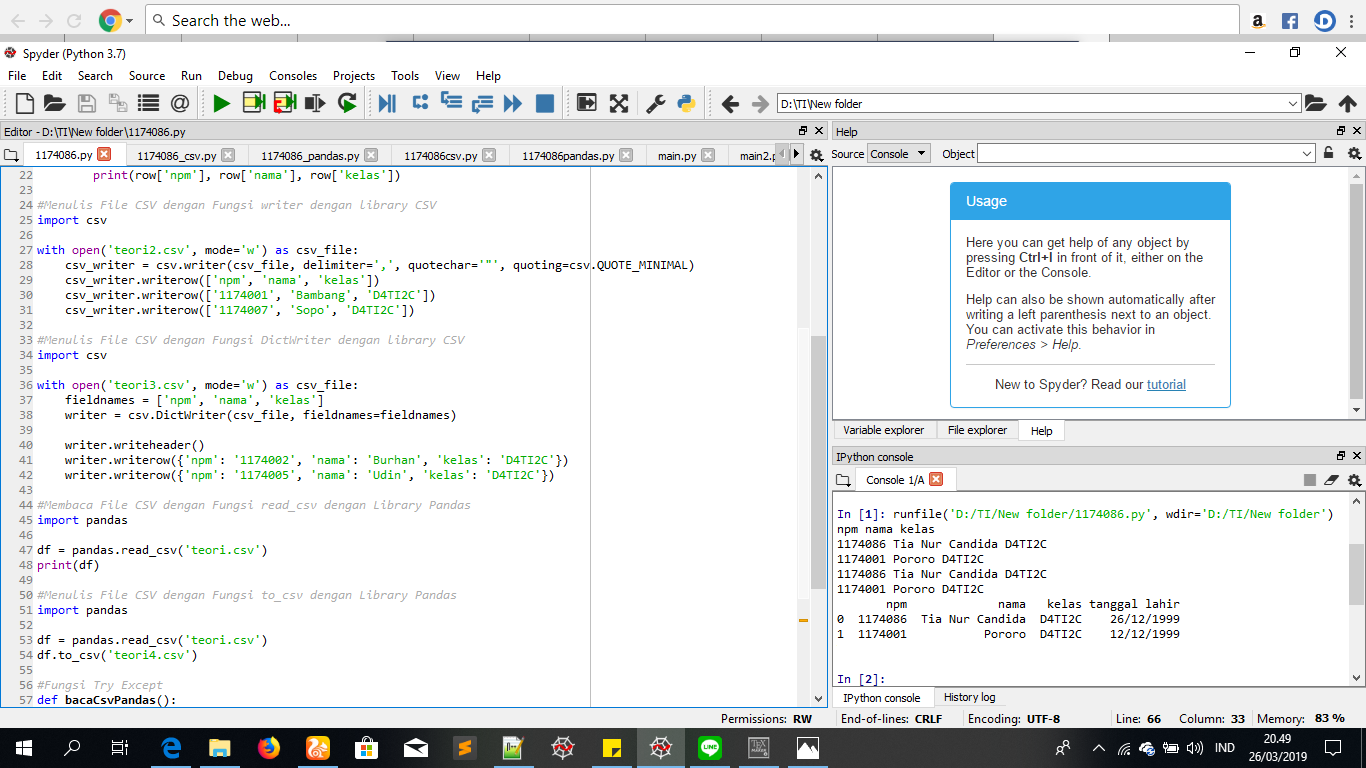
\includegraphics[width=10cm]{figures/4/1174086/k1.png}
	\centering
\end{figure}
\begin{figure}[H]
	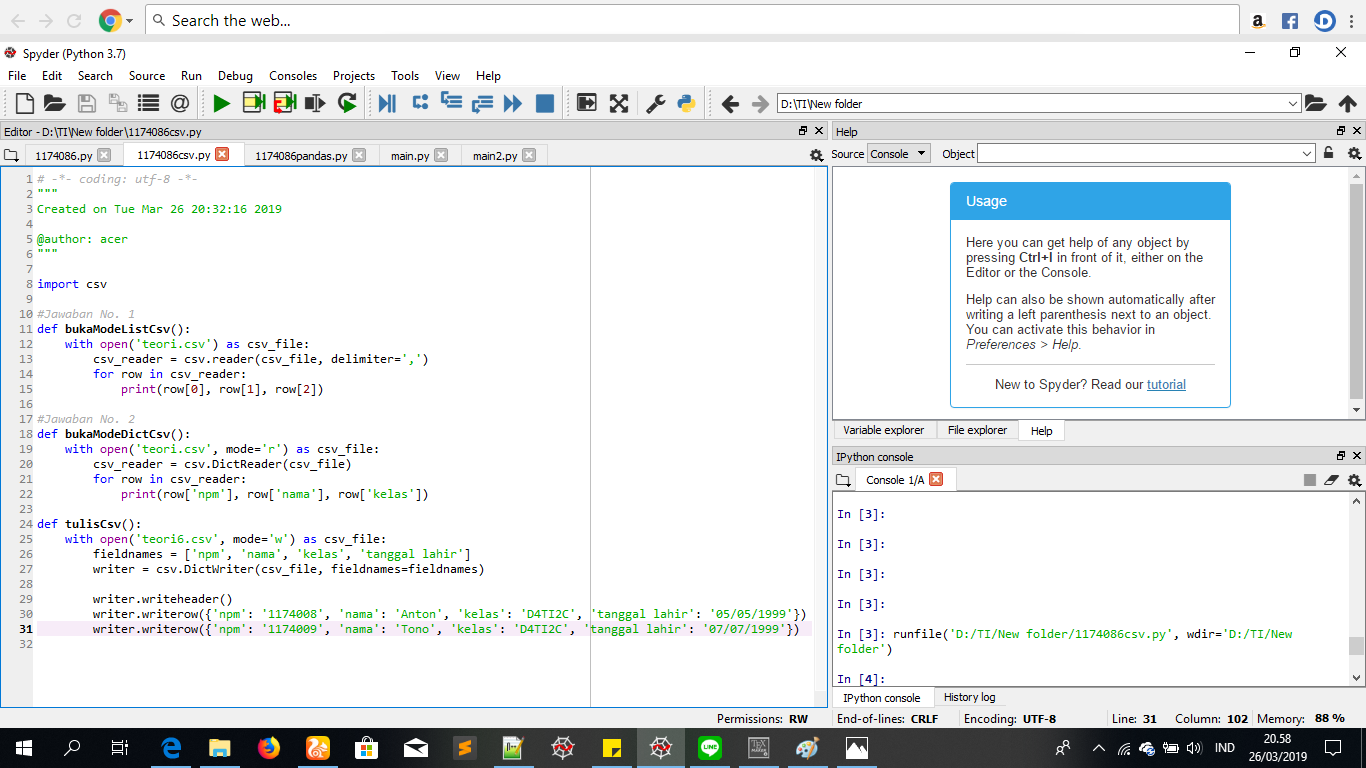
\includegraphics[width=10cm]{figures/4/1174086/k2.png}
	\centering
\end{figure}
\begin{figure}[H]
	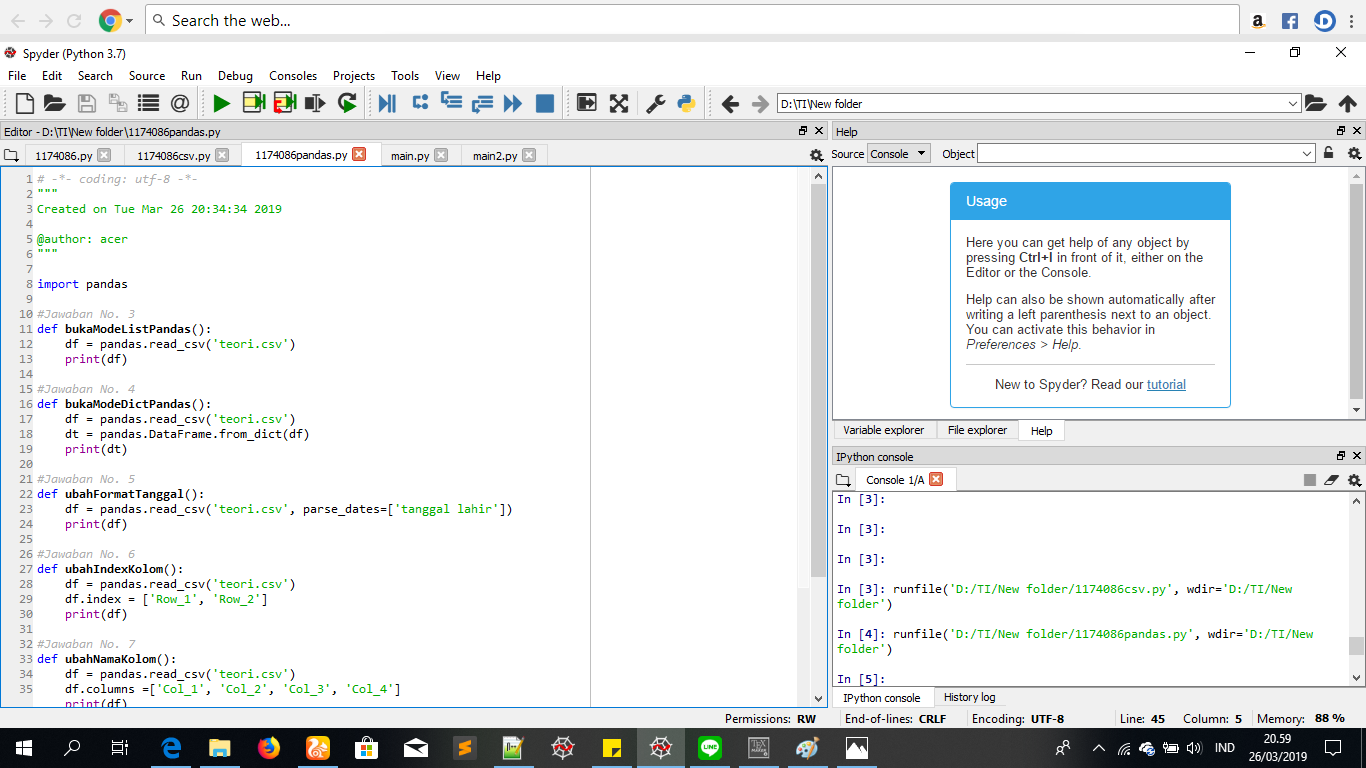
\includegraphics[width=10cm]{figures/4/1174086/k3.png}
	\centering
\end{figure}
\begin{figure}[H]
	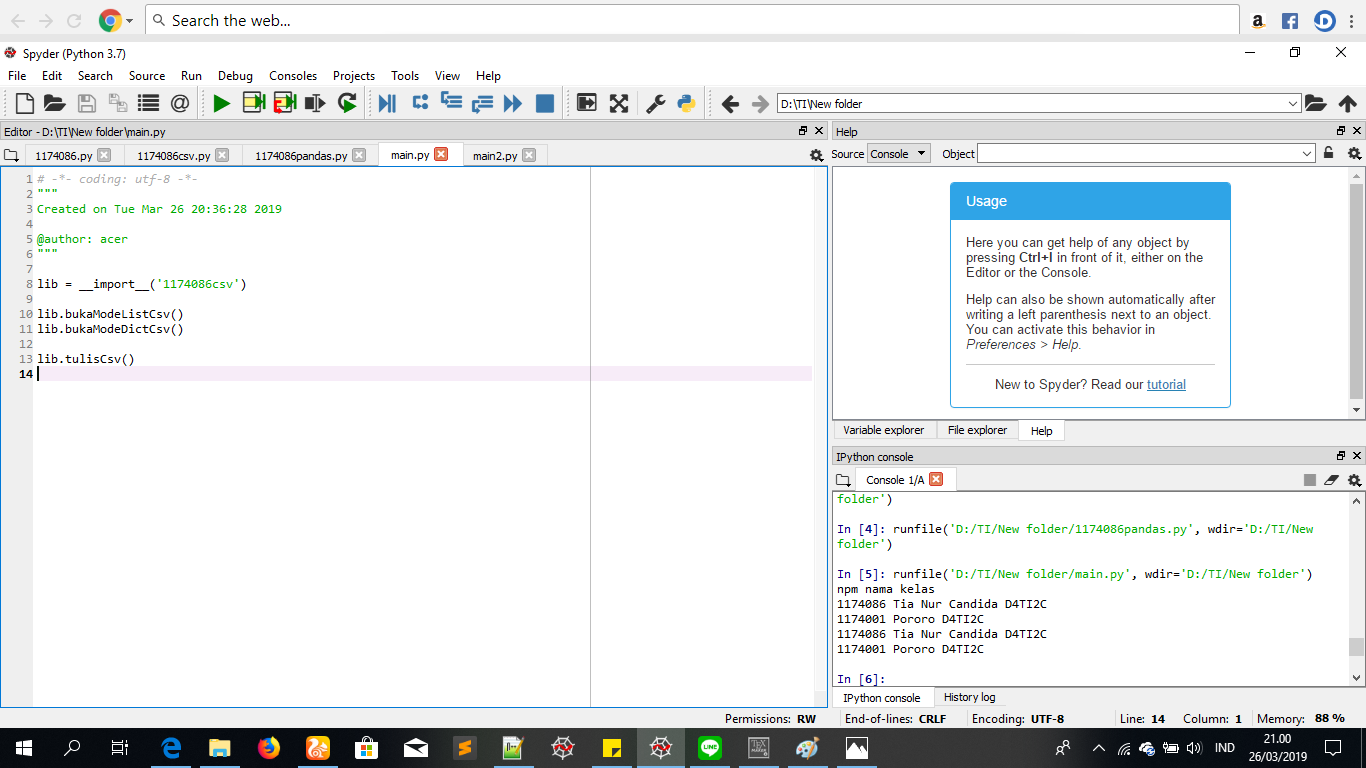
\includegraphics[width=10cm]{figures/4/1174086/k4.png}
	\centering
\end{figure}
\begin{figure}[H]
	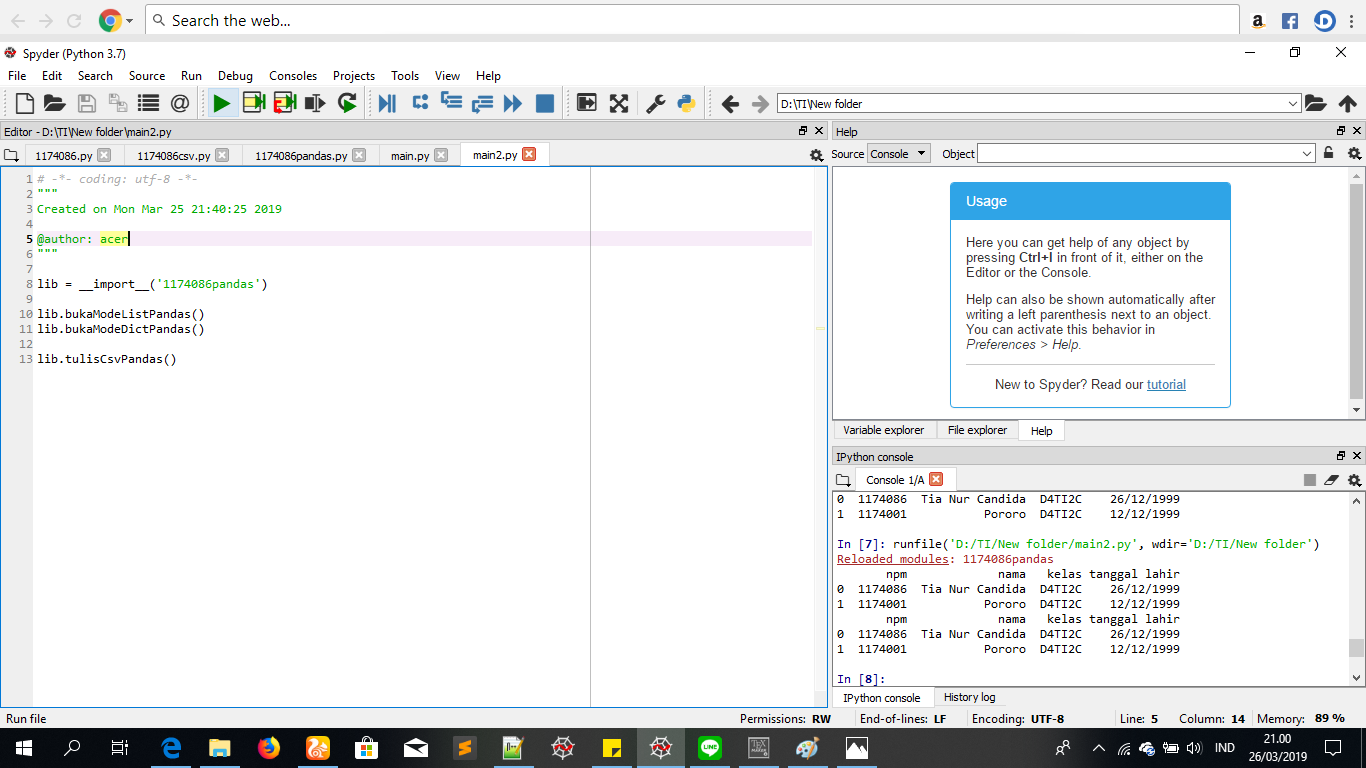
\includegraphics[width=10cm]{figures/4/1174086/k5.png}
	\centering
\end{figure}

\textbf{Cek Plagiat}
\begin{figure}[H]
	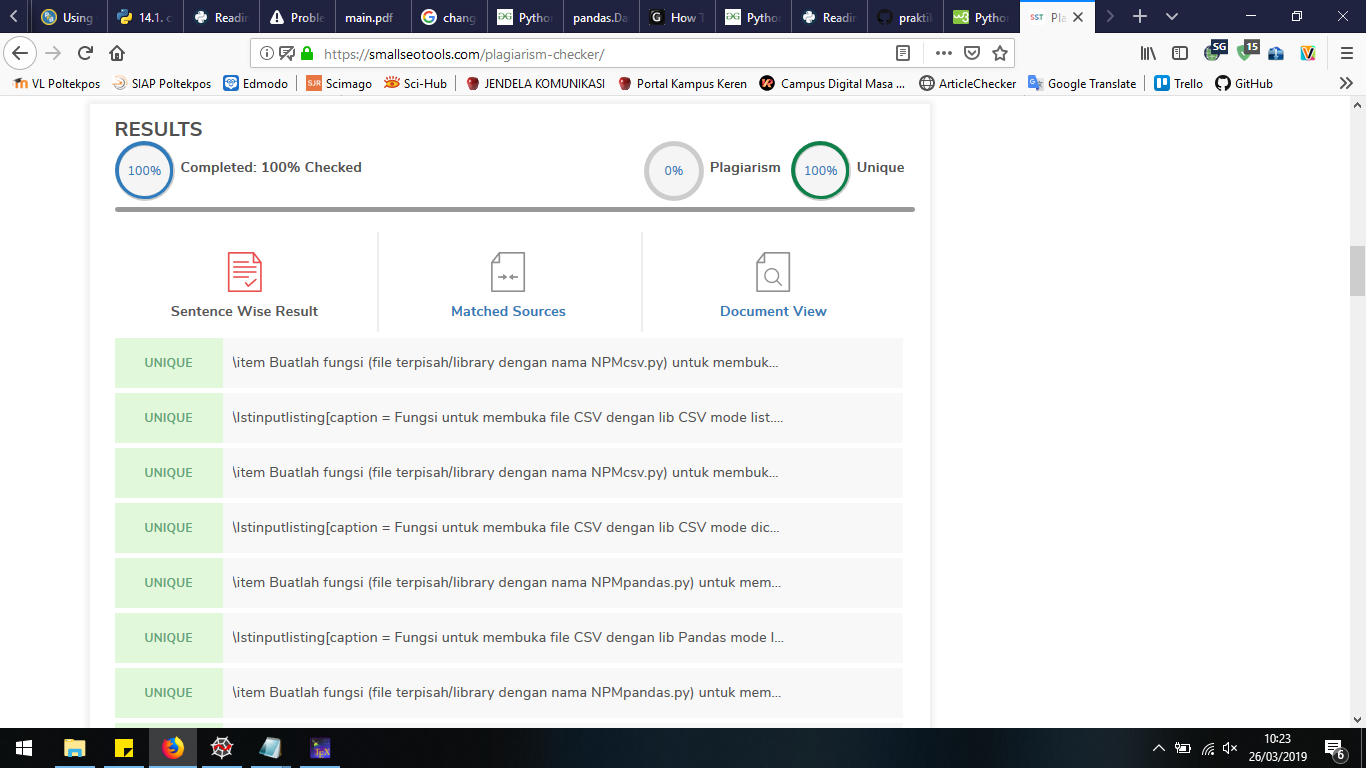
\includegraphics[width=10cm]{figures/4/1174086/plagiatketrampilan.png}
	\centering
\end{figure}
\section{Penanganan Error}
	\begin{enumerate}
	\item Tuliskan  peringatan  error  yang  didapat  dari  mengerjakan  praktek  keempat  ini, dan  jelaskan  cara  penanganan  error  tersebut.   dan  Buatlah  satu  fungsi  yang menggunakan gunakan try except untuk menanggulangi error tersebut.
	\end{enumerate}
	Peringatan error di praktek keempat ini, yaitu:
	\begin{itemize}
		\item Syntax Errors
		Syntax Errors adalah suatu keadaan saat kode python mengalami kesalahan penulisan. Solusinya adalah memperbaiki penulisan kode yang salah.
		
		\item Name Error
		NameError adalah exception yang terjadi saat kode melakukan eksekusi terhadap local name atau global name yang tidak terdefinisi. Solusinya adalah memastikan variabel atau function yang dipanggil ada atau tidak salah ketik.
		
		\item Type Error
		TypeError adalah exception yang akan terjadi apabila pada saat dilakukannya eksekusi terhadap suatu operasi atau fungsi dengan type object yang tidak sesuai. Solusi dari error ini adalah mengkoversi varibelnya sesuai dengan tipe data yang akan digunakan.
	\end{itemize}
	
	Fungsi yang menggunakan try except
	\lstinputlisting[caption= Fungsi yang menggunakan try except .,firstline=55, lastline=67]{src/4/1174086/1174086.py}
\end{enumerate}

\textbf{Kode Program}
\begin{figure}[H]
	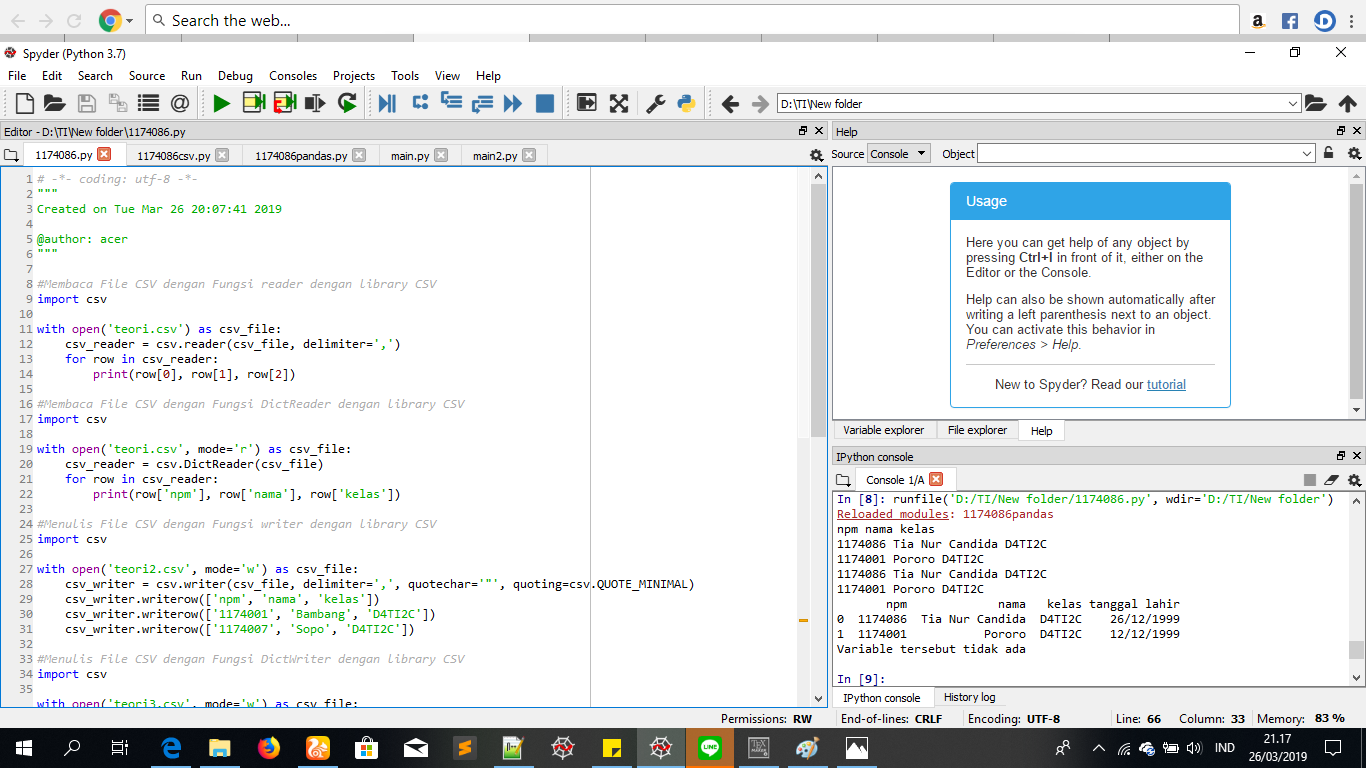
\includegraphics[width=10cm]{figures/4/1174086/p1.png}
	\centering
\end{figure}

\textbf{Cek Plagiat}
\begin{figure}[H]
	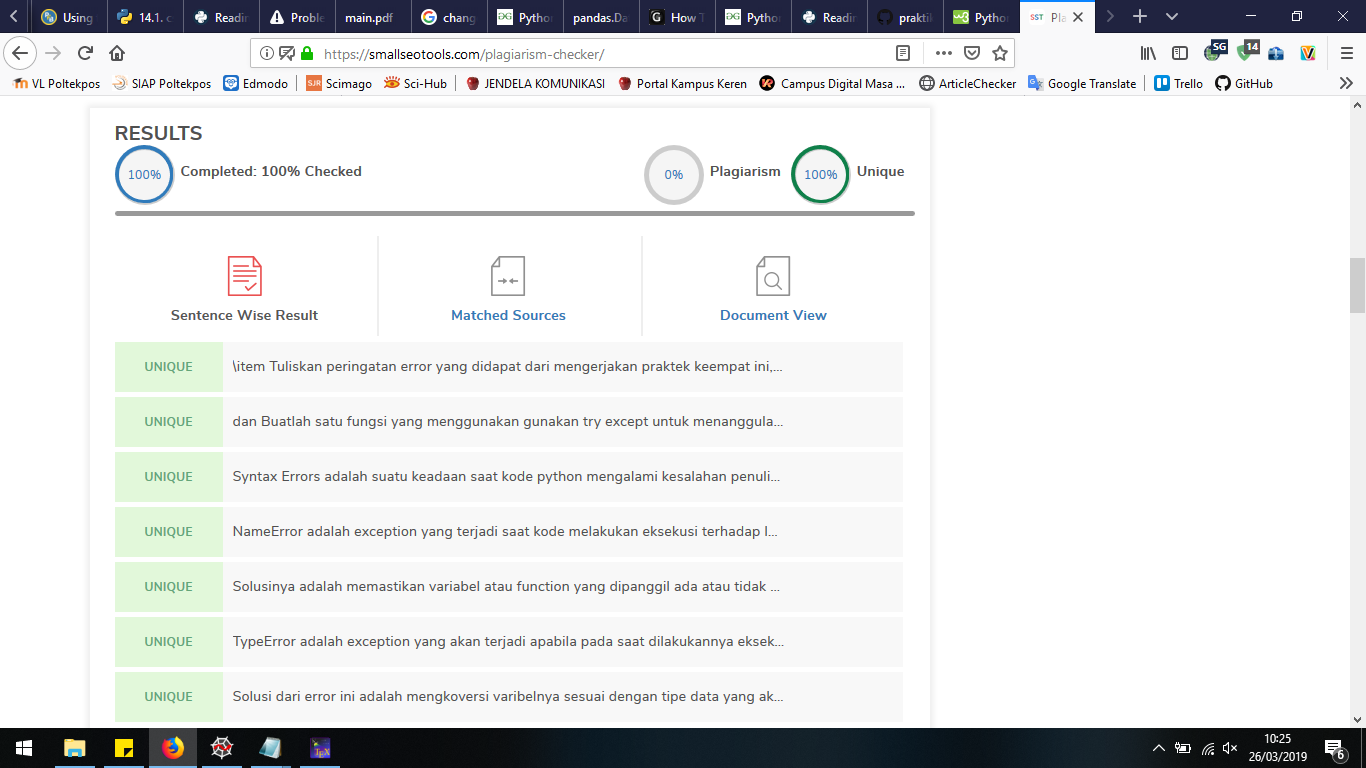
\includegraphics[width=10cm]{figures/4/1174086/plagiatpenanganan.png}
	\centering
\end{figure}

%%%%%%%%%%%%%%%%%%%%%%%%%%%%%%%%%%%%%%%%%%%%%%%%%%%%%%%%%%%%%%%%%%%%%%%%%%%%%%%%%%%%%%%%%%%%%%%%%%%%%%%

%%%%%%%%%%%%%%%%%%%%%%%%%%%%%%%%%%%%%%%%%%%%%%%%%%%%%%%%%%%%%%%%%%%%%%%%

\section{Difa Al Fansha}
\subsection{Soal Nomor 1}
Buatlah fungsi untuk membuka file csv dengan lib csv mode list

\lstinputlisting[firstline=10, lastline=17]{src/4/1174076/Praktek/coba.csv}
\begin{figure}[!htbp]
  \centering
  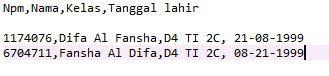
\includegraphics[height=3cm]{figures/4/1174076/Praktek/coba.png}
  \caption{Tampilan Kode Coba.scv}
\end{figure}

\lstinputlisting[firstline=10, lastline=17]{src/4/1174076/Praktek/1174076_csv.py}
\begin{figure}[!htbp]
  \centering
  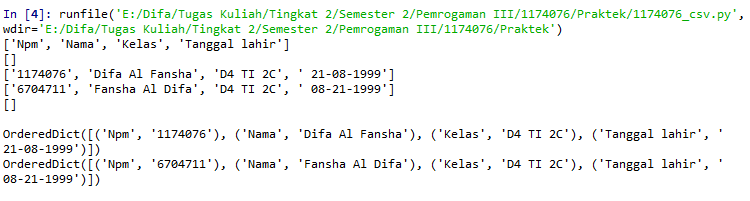
\includegraphics[height=3cm]{figures/4/1174076/Praktek/1174076_csv.png}
  \caption{Output csv mode directoy, untuk Nomor 1,2,dan 8}
\end{figure}


\subsection{Soal Nomor 2}
Buatlah fungsi untuk membuka file csv dengan lib csv mode dictionary
\lstinputlisting[firstline=21, lastline=27]{src/4/1174076/Praktek/1174076_csv.py}

\subsection{Soal Nomor 3}
Buatlah fungsi untuk membuka file csv dengan lib pandas mode list
\lstinputlisting[firstline=11, lastline=15]{src/4/1174076/Praktek/1174076_pandas.py}
\begin{figure}[!htbp]
  \centering
  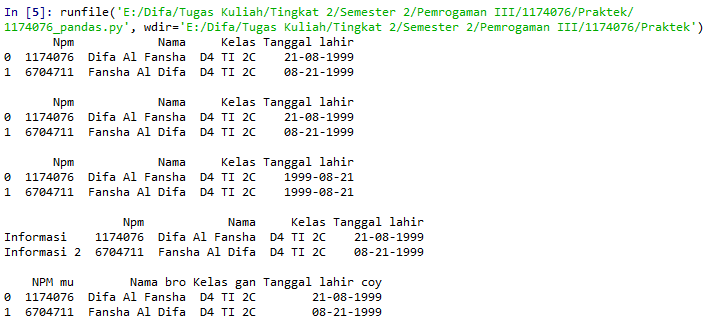
\includegraphics[height=3cm]{figures/4/1174076/Praktek/1174076_pandas.png}
  \caption{Output pandas mode list Nomor 3,4,5,6,7 dan 9}
\end{figure}

\subsection{Soal Nomor 4}
Buatlah fungsi untuk membuka file csv dengan lib pandas mode dictionary
\lstinputlisting[firstline=18, lastline=23]{src/4/1174076/Praktek/1174076_pandas.py}

\subsection{Soal Nomor 5}
Buat fungsi baru untuk mengubah format tanggal menjadi standar dataframe
\lstinputlisting[firstline=26, lastline=30]{src/4/1174076/Praktek/1174076_pandas.py}

\subsection{Soal Nomor 6}
Buat fungsi baru untuk mengubah index kolom
\lstinputlisting[firstline=33, lastline=38]{src/4/1174076/Praktek/1174076_pandas.py}

\subsection{Soal Nomor 7}
Buat fungsi baru untuk mengubah atribut atau nama kolom
\lstinputlisting[firstline=41, lastline=46]{src/4/1174076/Praktek/1174076_pandas.py}

\subsection{Soal Nomor 8}
Buat program main yang menggunakan library NPM csv yang membuat dan membaca file csv
\lstinputlisting[firstline=8, lastline=14]{src/4/1174076/Praktek/main.py}
\begin{figure}[!htbp]
  \centering
  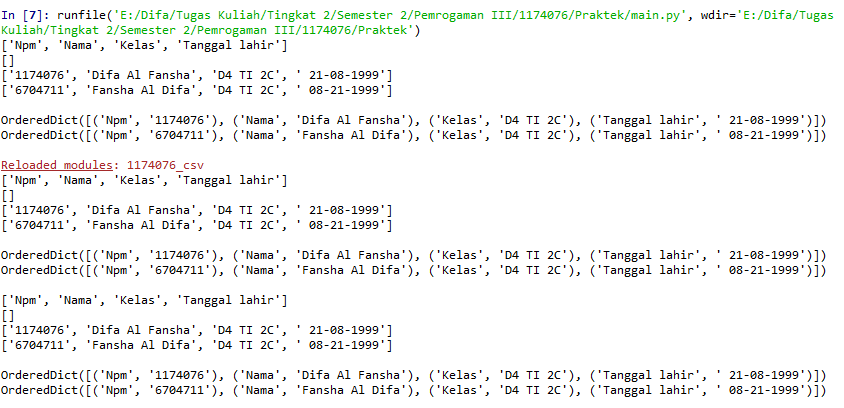
\includegraphics[height=3cm]{figures/4/1174076/Praktek/main.png}
  \caption{Output main.py}
\end{figure}

\lstinputlisting[firstline=30, lastline=39]{src/4/1174076/Praktek/1174076_csv.py}

\lstinputlisting[firstline=1, lastline=5]{src/4/1174076/Praktek/buatfile.csv}
\begin{figure}[!htbp]
  \centering
  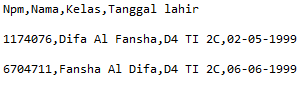
\includegraphics[height=3cm]{figures/4/1174076/Praktek/buatfile.png}
  \caption{Tampilan Koe buatfile.csv}
\end{figure}


\subsection{Soal Nomor 9}
Buat program main2.py yang menggunakan library NPM pandas.py yang membuat dan membaca file csv

\lstinputlisting[firstline=8, lastline=14]{src/4/1174076/Praktek/main2.py}
\begin{figure}[!htbp]
  \centering
  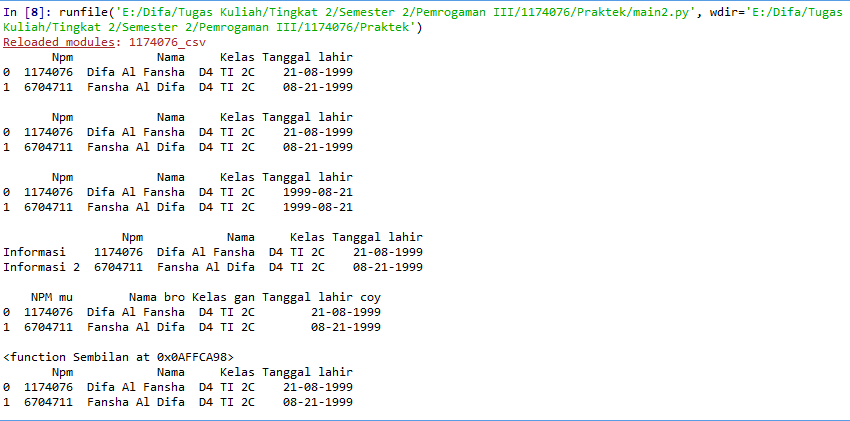
\includegraphics[height=3cm]{figures/4/1174076/Praktek/main2.png}
  \caption{Output pandas mode list Nomor 3,4,5,6,7 dan 9}
\end{figure}

\lstinputlisting[firstline=30, lastline=39]{src/4/1174076/Praktek/1174076_csv.py}

%%%%%%%%%%%%%%%%%%%%%%%%%%%%%%%%%%%%%%%%%%%%%%%%%%%%%%%%%%%%%%%%%%%%%%%%%%%%%%%%%%%%%%%%%%%%%%%%


%TEORI
\chapter{Komunikasi Perangkat Keras}
\section{D. Irga B. Naufal Fakhri}
\subsection{Pemahaman Teori}
\begin{enumerate}
\item Device Manager pada Windows dan folder /dev pada Linux

Device manager adalah system tools yang fungsinya untuk mengidentifikasi dan mengelola hardware serta driver yang diperlukan oleh hardware yang dihubungkan. Device Manager juga bisa mengenali hardware dan menginstall drivernya secara otomatis, tapi kalo driver dari hardware tersebut tidak ada pada koleksi driver Windows, maka Device Manager akan memberikan notifikasi dan tanda khusus bahwa hardware tersebut membutuhkan driver terpisah agar bisa terinstall dengan benar.

/dev pada Linux merupakan direktori yang berfungsi untuk menyimpan konfigurasi device atau hardware dari sistem, seperti harddisk (hda, sda), terminal (tty) dll.

\item Jelaskan langkah-langkah instalasi driver dari arduino

Apabila anda menggunakan Arduino versi original maka drivernya akan diinstall saat anda menginstall Arduino IDE saat anda menhubungkan Arduino anda ke PC menggunakan kabel USB. Jika anda menggunakan Arduino Uno SMD Clone seperti saya maka anda harus menginstall drivernya terlebih dahulu setelah menginstall Arduino Uno, Caranya:
	\begin{itemize}
	\item Buka program setup.exe pada folder DRIVER1
	\begin{figure}[ht!]
		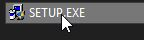
\includegraphics[width=5cm]{figures/5/1174066/0.jpg}
		\centering
		\caption{Setup}
	\end{figure}
	
	\item Setelah itu klik Install
	\begin{figure}[ht!]
		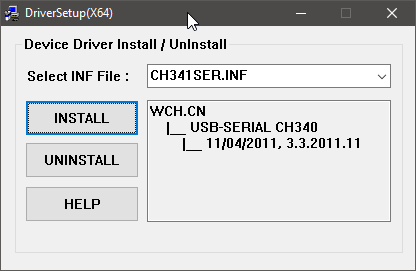
\includegraphics[width=5cm]{figures/5/1174066/1.png}
		\centering
		\caption{Instalasi}
	\end{figure}

	\item Setelah muncul seperti dibawah ini tekan OK
	\begin{figure}[ht!]
		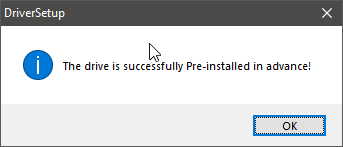
\includegraphics[width=5cm]{figures/5/1174066/2.png}
		\centering
		\caption{Instalasi Berhasil}
	\end{figure}

	\item Hubungkan Arduino ke PC, lalu buka device manager\begin{figure}[ht!]
		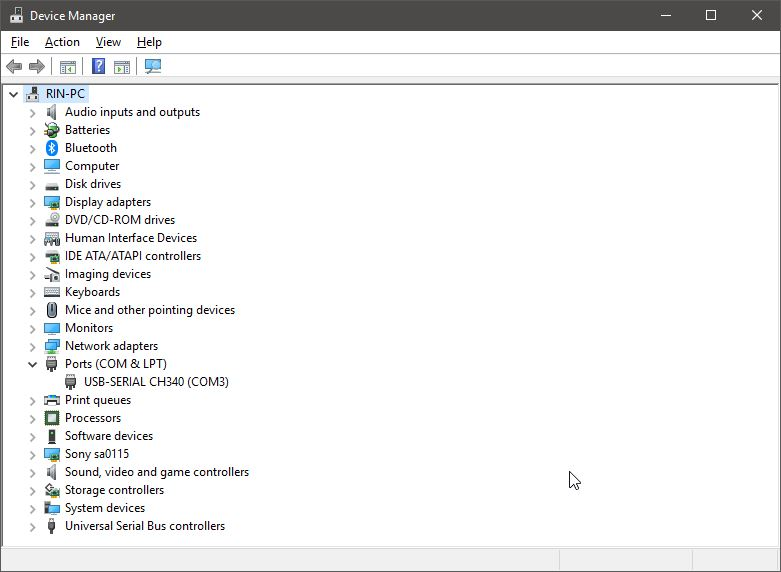
\includegraphics[width=5cm]{figures/5/1174066/3.jpg}
		\centering
		\caption{Device Manager}
	\end{figure}

	\item Lalu pilih pada bagian port apabila seperti ini maka driver arduino telah terinstall\begin{figure}[ht!]
		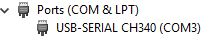
\includegraphics[width=5cm]{figures/5/1174066/4.jpg}
		\centering
		\caption{Arduino Terdeteksi}
	\end{figure}
	
	\end{itemize}

\item Jelaskan bagaimana cara membaca baudrate dan port dari komputer yang sudah terinstall driver

Cara membaca baudrate adalah dengan cara membuka arduino ide lalu mengclik serial monitor yang iconnya seperti kaca pembesar(Cari). 
Untuk mengecek port kita bisa melihatnya melalu device manager pada bagian ports, yang ada tulisan COMXX (XX adalah angka dari COM) itu adalah portnya
	
\item Jelaskan sejarah library pyserial

pySerial adalah modul API Python untuk mengakses port serial. pySerial menyediakan API yang seragam di berbagai sistem operasi, termasuk Windows, Linux, dan BSD.

\item Jelaskan fungsi-fungsi apa saja yang dipakai dari library pyserial

	\begin{itemize}
	\item Serial()
	
	Berfungsi untuk membuka port serial.
	
	\item Write()
	
	Berfungsi untuk mengirimkan data string ke port serial dan mengembalikan nomor bytes yang terkirim.
	
	\item Read(size)
	
	Berfungsi untuk membaca data dari port serial.
	
	\item Readline(size)
	
	Berfungsi untuk membaca line sampai line terakhir (EOL). 
	
	\item Close()
	
	Berfungsi untuk menutup pembacaan port serial.
	\end{itemize}

\item Jelaskan kenapa butuh perulangan dan tidak butuh perulangan dalam membaca serial

Perulangan dalam python berfungsi untuk mengulangi kode/perintah yang ada didalam perulangan tersebut. ada dua macam perulangan pada python, yang pertama for dan yang kedua while.
Perbedaan for dan while adalah for yaitu perulangan yang menghitung (Counted Loop) sedangkan while adalah perulangan yang tidak terhitung (Uncounted Loop). Penggunakan for itu biasanya jika untuk mengulangi kode yang akan ditentukan berapa kali diulangnya sedangkan while digunakan jika ada syarat tertentu untuk mengulangi kode itu dan tidak menentu berapa banyak perulangannya.
Mengapa diperlukan perulangan, karena agar data yang dibaca tidak hanya satu kali saja namun berkali kali, dengan adanya perulangan kita bisa membaca datanya berulang kali. Sehingga data yang kita baca dapat muncul lebih dari satu. Sedangkan kalau kita tidak memakai perulangan maka data yang muncul hanya satu.

\item Jelaskan bagaimana cara membuat fungsi yang mengunakan pyserial

Pembuatan fungsi sama seperti pembuatan fungsi seperti biasanya namun method dari pyserial dimasukkan kedalam fungsi dan dipanggil fungsi yang kita buat tadi
\lstinputlisting[firstline=7, lastline=14]{src/5/1174066/Teori/1174066.py}

\item Scan Plagiarisme
\begin{figure}[ht!]
	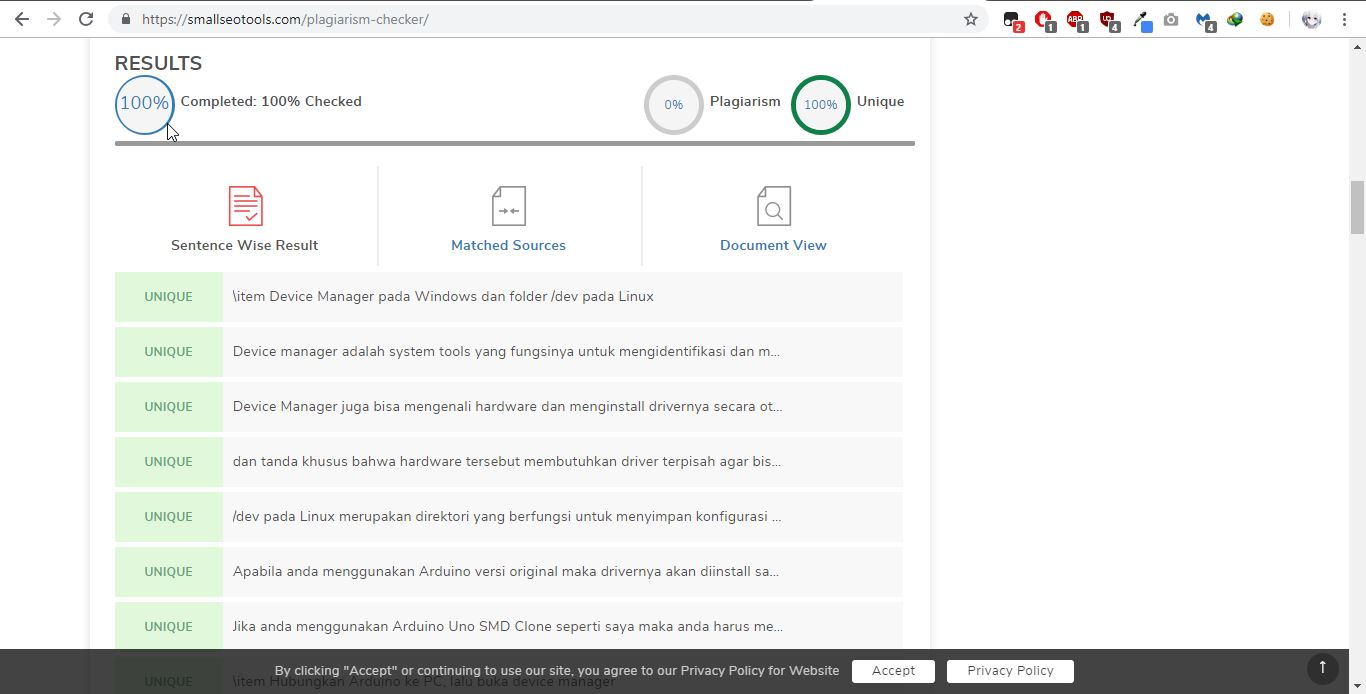
\includegraphics[width=5cm]{figures/5/1174066/plagiat.jpg}
	\centering
	\caption{Plagiarisme}
\end{figure}
\end{enumerate}

%%%%%%%%%%%%%%%%%%%%%%%%%%%%%%%%%%%%%%%%%%%%%%%%%%%%%%%%%%%%%%%%%%%%%%%%%
\section{Difa Al Fansha}
\subsection{Soal Nomor 1}
Apa itu fungsi device manager di windows dan folder /dev di linux?\\
Jawab :
\begin{itemize}
\item Fungsi Device Manager di Sistem Operasi Windows
\end{itemize}
Device manager merupakan program yang mengatur device atau perangkat yang terhuung dengan komputer / laptop.
\begin{itemize}
\item Fungsi Folder /dev di Sistem Operasi Linux
\end{itemize}
Device manager pada linux berada pada folder /dev yang mempunyai arti device. folder ini berisi konfigurasi device pada sistem.

\subsection{Soal Nomor 2}
Jelaskan langkah-langkah instalasi driver dari arduino!\\
Jawab :
\begin{enumerate}
\item Download Software IDE Arduino di https://www.arduino.cc/en/Main/Software
\item Setelah di download jalankan software tersebut.

\item Pilih I Agree.
\begin{figure}[!htbp]
  \centering
  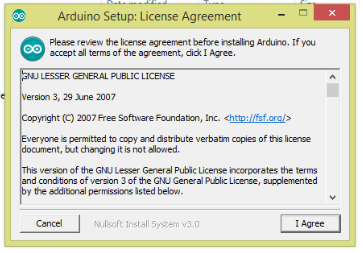
\includegraphics[height=8cm]{figures/5/1174076/Teori/1.PNG}
  \caption{Licence Agreement}
\end{figure}

\item Lalu Next.
\begin{figure}[!htbp]
  \centering
  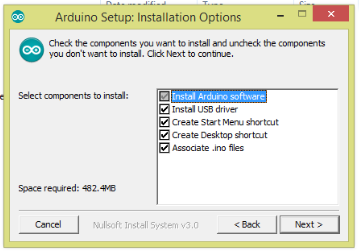
\includegraphics[height=8cm]{figures/5/1174076/Teori/2.PNG}
  \caption{Installation Options}
\end{figure}

\item Pilih directory, lalu tekan Install.
\begin{figure}[!htbp]
  \centering
  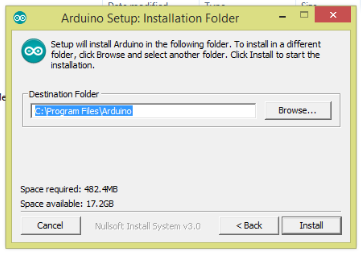
\includegraphics[height=8cm]{figures/5/1174076/Teori/3.PNG}
  \caption{Installation Folder}
\end{figure}

\item Tunggu hingga proses selesai
\begin{figure}[!htbp]
  \centering
  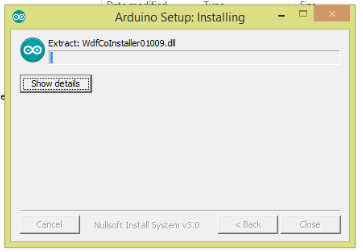
\includegraphics[height=8cm]{figures/5/1174076/Teori/4.PNG}
  \caption{Installation }
\end{figure}

\item Jika sudah selesai, tekan close
\begin{figure}[!htbp]
  \centering
  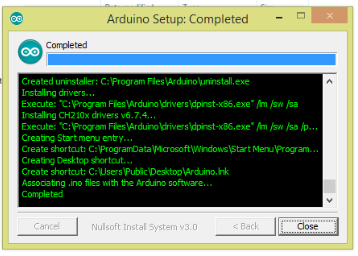
\includegraphics[height=8cm]{figures/5/1174076/Teori/5.PNG}
  \caption{Installing}
\end{figure}
\end{enumerate}

\subsection{Soal Nomor 3}
Jelaskan bagaimana cara membaca baud rate dan port dari komputer yang sudah
terinstall driver! \\
Jawab :\\
baud rate dan port akan langsung terbaca saat arduino dicolokkan ke komputer, sistem akan membaca informasi device yang terhubung.

\subsection{Soal Nomor 4}
Jelaskan sejarah library pyserial!
Jawab : \\
Salah satu cara untuk melakukan komunikasi melalui serial menggunakan python adalah dengan menggunakan modul pyserial. PySerial diluncurkan pada tahun 2002.

\subsection{Soal Nomor 5}
Jelaskan fungsi-fungsi apa saja yang dipakai dari library pyserial!\\
Jawab :\\
\begin{itemize}
\item stop() berguna untuk menghentikan program yang berjalan.
\item readline() berguna untuk membaca sebuah string dari port serial.
\item read(size)berguna untuk membaca jumlah byte dari port serial.
\item close()berguna untuk menutup port serial.
\end{itemize}

\subsection{Soal Nomor 6}
Jelaskan kenapa butuh perulangan dan tidak butuh perulangan dalam membaca serial!\\
Jawab :\\
\begin{itemize}
\item Perulangan
\end{itemize}
Perulangan diperlukan untuk untuk mengulangi perintah agar lebih mudah dan tidak terjadi penumpukan kodingan. Perulangan dijalankan jika kondisi benar dan akan berhenti jika kondisi salah.

\begin{itemize}
\item Tidak membutuhkan perulangan
\end{itemize}
Apabila perintah dijalankan sekali, kita tidak memerlukan perulangan.

\subsection{Soal Nomor 7}
Jelaskan bagaimana cara membuat fungsi yang menggunakan pyserial!\\
Jawab :\\
Definisikan nama fungsi dengan cara def namaFungsi(): lalu masukkan isi fungsi

%%%%%%%%%%%%%%%%%%%%%%%%%%%%%%%%%%%%%%%%%%%%%%%%%%%%%%%%%%%%%%%%%%%%%%%%%%%%%%%%%%%%%%%%%%%%%%%%%%%%%%%%%%%%%%%%%%%%%%%%%%

\section{Fanny Shafira Damayanti | 1174069}
\subsection{Pemahaman Teori}
\begin{enumerate}
\item Fungsi Device manager di Windows dan folder /dev di Linux

Device Manager di Windows berfungsi untuk mengelola semua Hardware yang berada di Windows.

Folder /dev berisikan file device pada Linux.

\item Langkah-langkah Instalasi driver dari arduino

\begin{itemize}
\item Download Software Arduino IDE
\item Hubungkan port USB Arduino ke port pc.
\item setelah itu pc akan mendeteksi driver baru

\begin{figure}[ht!]
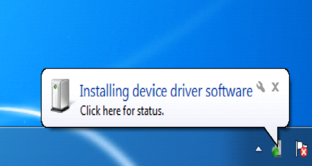
\includegraphics[width=5cm]{figures/5/1174069/1fny.png}
\centering
		\caption{Driver baru}
\end{figure}
	
\item Buka device manager

\begin{figure}[ht!]
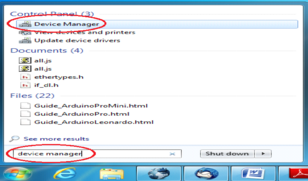
\includegraphics[width=5cm]{figures/5/1174069/2fny.png}
\centering
		\caption{Buka device manager}
\end{figure}
	
	
\item setelah itu, cari "Unknown device"

\begin{figure}[ht!]
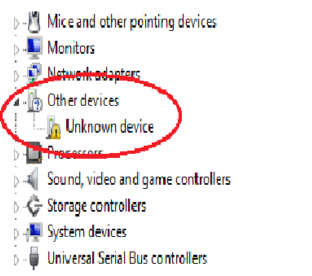
\includegraphics[width=5cm]{figures/5/1174069/3fny.png}
\centering
		\caption{klik "unknown device"}
\end{figure}
	
\item Klik kanan pada "Unknown device" lalu klik Update driver software

\begin{figure}[ht!]
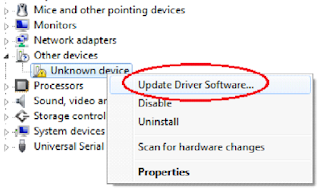
\includegraphics[width=5cm]{figures/5/1174069/4fny.png}
\centering
		\caption{Klik update driver software}
\end{figure}
	
\item Pilih Browse my computer for driver software

\begin{figure}[ht!]
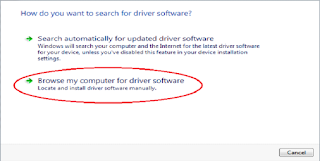
\includegraphics[width=5cm]{figures/5/1174069/5fny.png}
\centering
		\caption{Pilih browse}
\end{figure}
	
\item Cari folder installan Arduino nya

\begin{figure}[ht!]
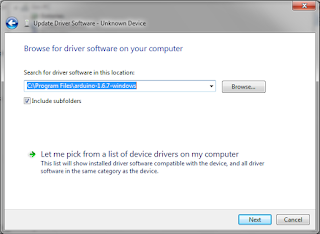
\includegraphics[width=5cm]{figures/5/1174069/6fny.png}
\centering
		\caption{Cari folder instalasinya}
\end{figure}
	
\item Lalu klik next


	
\item setelah itu klik install
\begin{figure}[ht!]
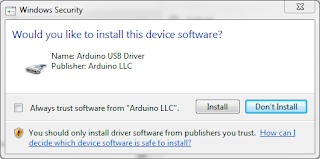
\includegraphics[width=5cm]{figures/5/1174069/7fny.png}
\centering
		\caption{install}
\end{figure}

\item Arduino telah berhasil di install

\begin{figure}[ht!]
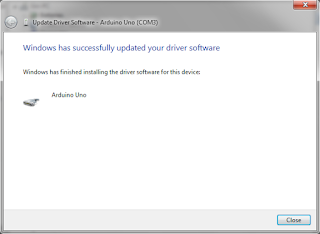
\includegraphics[width=5cm]{figures/5/1174069/8fny.png}
\centering
\caption{selesai}
\end{figure}
	
\end{itemize} 

\item Cara membaca baudrate dan port dari komputer yang sudah terinstall driver

Untuk membaca baudrate dan port yaitu dengan cara :
\begin{itemize}
\item menginstall Arduino IDE
\item setelah itu buka menu serial monitor yang berada di tab tools
\item lalu akan terlihat baudrate dan port yang sedang digunakan.
\end{itemize}

\item Sejarah library pyserial
PySerial merupakan sebuah library yang digunakan untuk komunikasi ke port serial terutama untuk mikrokontroller. PySerial pertama kali diluncurkan pada tahun 2002 yang makin berkembang dalam setiap versinya hingga tahun 2017 lalu.

\item Fungsi-fungsi yang di pakai dari libarary pyserial

\begin{itemize}
			\item \begin{verbatim}stop()\end{verbatim} : untuk menghentikan pembacaan program
			\item \begin{verbatim}serial.to_bytes(sequence)\end{verbatim} : berfungsi untuk mengubah sequence ke dalam bytes agar dapat dikirim ke dalam arduino.
			\item \begin{verbatim}close()\end{verbatim} : untuk menutup port dan menghentikan pembacaan program
		\end{itemize}

\item kenapa butuh perulangan dan tidak butuh perulangan dalam membaca serial

Karena perulangan digunakan untuk membaca seluruh data pada serial yang ada setiap baris. Perulangan digunakan agar data dapat muncul secara terus menerus atau realtime. Sedangkan kalau tidak memakai perulangan, maka data hanya muncul satu kali, tidak berulang.

\item Cara membuat fungsi menggunakan pyserial

\lstinputlisting[firstline=7, lastline=14]{src/5/1174069/Teori/1174069_teori.py}

\item Scan Plagiarisme
\begin{figure}[ht!]
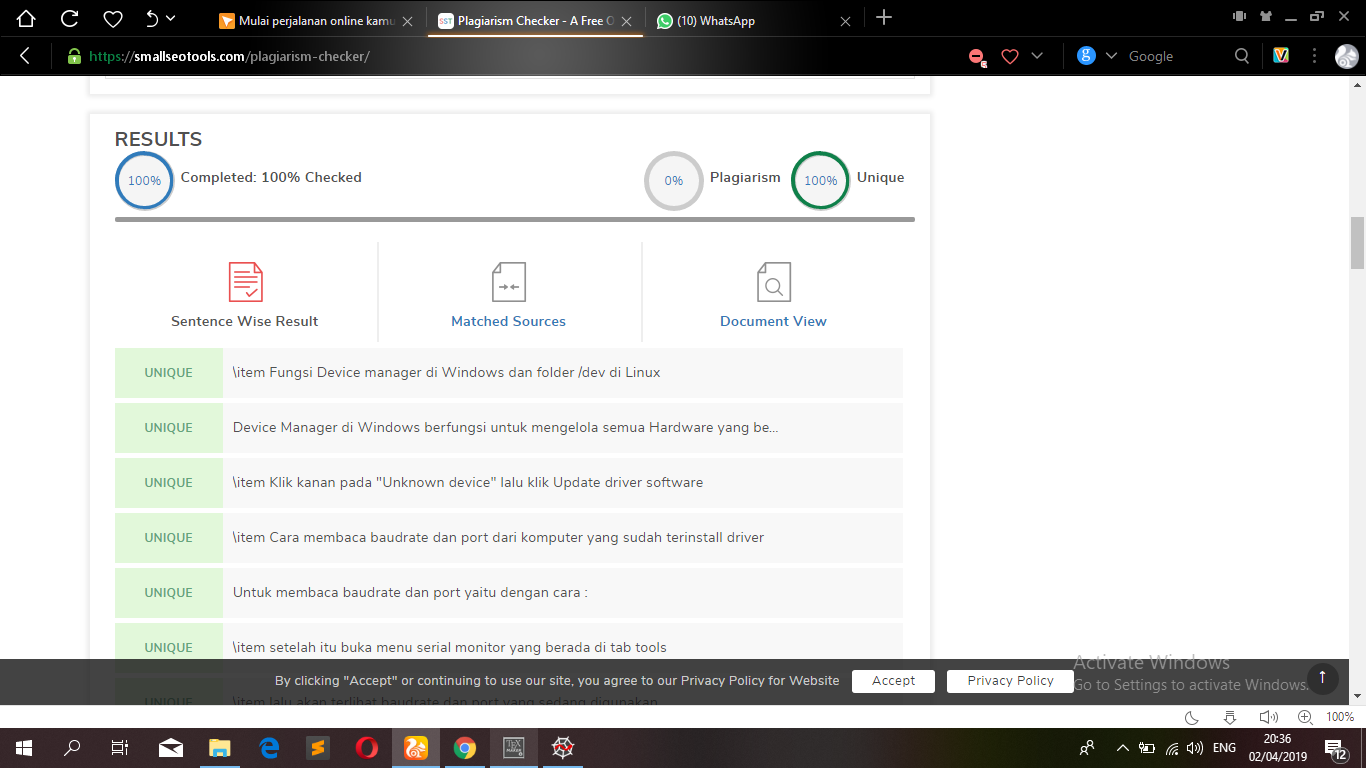
\includegraphics[width=5cm]{figures/5/1174069/plagiarisme.png}
\centering
\caption{plagiarisme}
\end{figure}
\end{enumerate}

%%%%%%%%%%%%%%%%%%%%%%%%%%%%%%%%%%%%%%%%%%%%%%%%%%%%%%%%%%%%%%%%%%%%%%%%%%%%%%%%%%%%%%%%%%%%%%%%%%%%%%%%%%%%%%%%%%%%

\section{Aulyardha Anindita | 1174054}
\subsection{Pemahaman Teori}
\begin{enumerate}

\item Fungsi Device Manager dan folder /dev
\begin{itemize}
\item Fungsi Device Manager\\
Device manager dalam windows merupakan perluasan dari microsoft management console. Device manager mampu menampilkan seluruh hardware yang bisa di inisialisasi (dikenali) oleh windows. Device manager disini memiliki beberapa fungsi diantaranya :\\
a.	Menunjukkan status suatu hardware\\
b.	Menunjukkan informasi detail suatu hardware\\
c.	Mengelola driver hardware\\
d.	Disable dan enable hardware\\
e.	Memberikan pesan error terjadinya problem status device\\
\item Fungsi Folder /dev\\
Folder/dev adalah suatu representasi dari drive yang terhubung ke dalam sistem operasi linux dan sistem mengganggapnya sebagai file-file direktori. Biasanya sering ditampilkan direktori seperti /dev/sdal yang mewakili Drive SATA pertama dalam sistem.
\end{itemize}

\item Langkah-langkah instalasi driver dari arduino
\begin{itemize}
\item Pertama, download dan instal terlebih dahulu Arduino IDE

\item Hubungkan port USB Arduino UNO ke Port USB PC, maka PC akan mendeteksi keberadaan perangkat baru dan akan muncul pop up berupa pesan install device driver software. Seperti pada gambar berikut :
\begin{figure}[ht!]
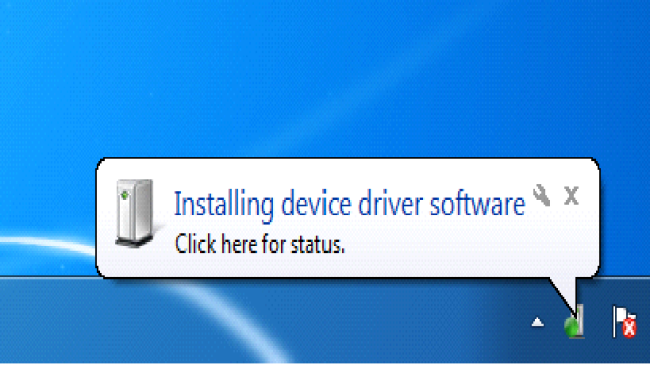
\includegraphics[width=5cm]{figures/5/1174054/1.png}
\centering
\caption{Setup}
\end{figure}

\item Dalam Windows tidak menyediakan menyediakan driver untuk Arduino Uno seperti yang terlihat pada gambar dibawah ini, sehingga proses instalasinya harus dilakukan secara manual.
\begin{figure}[ht!]
\includegraphics[width=5cm]{figures/5/1174054/2.png}
\centering
\caption{Instalasi}
\end{figure}

\item Selanjutnya, buka start windows kemudian ketikkan device manager lalu tekan enter, maka akan muncul device manager. Klik untuk menjalankan. Seperti pada gambar berikut :
\begin{figure}[ht!]
\includegraphics[width=5cm]{figures/5/1174054/3.png}
\centering
\caption{Search Device Manager}
\end{figure}

\item Kemudian Carilah Unknown device pada bagian Other device, biasanya terdapat tanda seru berwarna kuning hal itu disebabkan karena penginstallan tidak berjalan dengan sempurna.
\begin{figure}[ht!]
\includegraphics[width=5cm]{figures/5/1174054/4.png}
\centering
\caption{Unknown Device}
\end{figure}

\item Klik kanan pada “Unknown device” kemudian pilih Update Driver Software
\begin{figure}[ht!]
\includegraphics[width=5cm]{figures/5/1174054/5.png}
\centering
\caption{Update Driver Software}
\end{figure}

\item Pilih Browse my computer for driver software
\begin{figure}[ht!]
\includegraphics[width=5cm]{figures/5/1174054/6.png}
\centering
\caption{Mencari folder untuk driver software}
\end{figure}

\item  Arahkan lokasi folder ke folder arduino kemudian checkbox lalu centang include subfolders. setelah itu, Klik Next untuk melanjutkan instalasi driver.
\begin{figure}[ht!]
\includegraphics[width=5cm]{figures/5/1174054/7.png}
\centering
\caption{Lokasi folder}
\end{figure}

\item Kemudian lanjutkan dengan mengklik Install pada tampilan Windows Security
\begin{figure}[ht!]
\includegraphics[width=5cm]{figures/5/1174054/8.png}
\centering
\caption{Install PAda tampilan WIndows Security}
\end{figure}

\item Jika instalasi driver berhasil maka akan muncul Windows has successfully updated your driver software.
\begin{figure}[ht!]
\includegraphics[width=5cm]{figures/5/1174054/9.png}
\centering
\caption{Pesan Peringatan Berhasil}
\end{figure}

\item Perhatikan dan ingat nama COM Arduino Uno, karena nama COM ini yang akan digunakan untuk meng-upload program nantinya
\begin{figure}[ht!]
\includegraphics[width=5cm]{figures/5/1174054/10.png}
\centering
\caption{Peringatan COM Arduino Uno}
\end{figure}

\end{itemize}

\item Cara Membaca Baudrate dan Port

Cara membaca baudrate yaitu dengan membuka arduino ide yang telah diinstal lalu klik serial monitor dimana iconnya seperti kaca pembesar (cari).

Cara membaca port yaitu dengan melalui device manager pada bagian port yang terdapat tulisan COMXX dimana itu adalah portnya.

\item Sejarah Library Pyserial\\
PySerial merupakan sebuah library yang digunakan untuk komunikasi ke port serial terutama untuk mikrokontroller. PySerial pertama kali diluncurkan pada tahun 2002 yang makin berkembang dalam setiap versinya hingga tahun 2017 lalu. 

PySerial menyediakan antarmuka untuk berkomunikasi
melalui protokol komunikasi serial. Komunikasi serial adalah salah satu protokol komunikasi komputer tertua. Protokol komunikasi serial mendahului spesifikasi USB
yang digunakan oleh komputer dan perangkat keras lain seperti mouse, keyboard,dan webcam. USB adalah singkatan dari Universal Serial Bus. USB dan dibangun di atas dan memperluas antarmuka komunikasi serial asli.

\item Fungsi-fungsi pada Library Pyserial
\begin{itemize}
\item Serial(), berfungsi untuk membuka port serial
\item Write(), berfungsi untuk menulis data lewat port serial
\item readline(size), berfungsi untuk membaca sebuah string dari port serial
\item read(size), berfungsi untuk membaca jumlah byte dari port serial
\item close(), berfungsi untuk menutup port serial
\end{itemize}

\item Mengapa butuh perulangan dan tidak butuh perulangan dalam membaca serial\\
Ketika kita akan membaca serial di Arduino diperlukan perulangan yang berfungsi untuk membaca data secara berulang kali sehingga data yang muncul banyak. Sedangkan apabila tidak membutuhkan perulangan maka Arduino hanya akan membaca data satu kali saja.

\item Cara Membuat fungsi menggunakan Pyserial
\lstinputlisting[firstline=8, lastline=15]{src/5/1174054/Teori/1174054.py}

\item Cek Plagiarisme
\begin{figure}[ht!]
\includegraphics[width=5cm]{figures/5/1174054/plagiarisme.png}
\centering
\caption{Plagiarisme}
\end{figure}

\end{enumerate}

%%%%%%%%%%%%%%%%%%%%%%%%%%%%%%%%%%%%%%%%%%%%%%%%%%%%%%%%%%%%%%%%%%%%%%%%%%%%%%%%%%%%%%%%%%%%%%%%%%%%%%%%%%%%%%%%%%%%

\section{Nurul Izza Hamka | 1174062 | Teori}
\begin{enumerate}

\item Fungsi Device Manager di Windows dan Folder / Dev di Linux 
Device manager ini adalah untuk menampilkan semua hardware yang bisa dikenali oleh windows, tampilan di device manager ini sudah dikelompokkan dengan rapi serta teratur,dengan adanya device manager ini akan sangat membantu dalam memanajemen setiap hardware yang ada dalam windows. \\
Fungsi dari device manager ini adalah seperti :\\
1. Mengelola setiap driver didalam hardware,\\
2. Mengidentifikasi konfik yang terjadi dalam hardware,\\
3. Menunjukka setiap informasi secara detail suatu hardware,\\
4. Menampilkan status dalam hardware.\\
Sedangka pada Linux ia melihat hardware apa saja yang yang telah terpasang melalui command dan terminal ataupun secara Visual.

\item Langkah-Langkah Instalasi Driver dari Arduino : \\
Adapun langkah-langkah dalam menginstal arduino di Windows :\\
\begin{enumerate}
\item Pertama Hubungkan Port USB arduino UNO ke komputer atau Laptop,
	\item Setelah terhubung, laptop akan mengindentifikasi terlebih dahulu,
	\begin{figure}[ht!]
	\includegraphics[width=5cm]{figures/5/1174062/1.jpg}
	\centering
	\end{figure}
	\item Selanjutnya windows akan menginstall di driver,pastikan device manager kita telah terinstall,
	\begin{figure}[ht!]
	\includegraphics[width=5cm]{figures/5/1174062/2.png}
	\centering
	\end{figure}
	\item Di device manager padsa bagian Ports, akan muncul nama baru yaitu Arduino UNO,
	\item Klik kanan Arduino Uno tersebut kemudian pilih Update Driver Software, 
	\begin{figure}[ht!]
	\includegraphics[width=5cm]{figures/5/1174062/4.png}
	\centering
	\end{figure}
	\item Setelah itu Browser my Computer for driver software,lalu klik Next untuk install
	\begin{figure}[ht!]
	\includegraphics[width=5cm]{figures/5/1174062/5.png}
	\centering
	\end{figure}
	\item Jika berhasil, berarti Arduino telah berhasil di install.
	\begin{figure}[ht!]
	\includegraphics[width=5cm]{figures/5/1174062/7.png}
	\centering
	\end{figure}
\end{enumerate}
	

\item Cara membaca baudrate dan Port dari Komputer yang telah Terinstall Driver: \\
1. Buka device manager,\\
2. Pilih port (COM \& LPT),\\
3. Kemuadian double klik yang COM,\\
4. Pilih tab yang Port Setting, dan lihat pada Bit per Second,\\

Kemudian Cara Membaca Port Dari Komputer :
1. Buka device manager,\\
2. Pilih port (COM \& LPT),\\
3. Selanjutnya akan muncul jika port arduino telah terbaca oleh PC.\\

\item Sejarah Library Pyserial:
Pyserial adalah perpustakaan yang meyediakan  dukungan untuk sebuah koneksi serial "RS-232" melalui berbagi perangkat yang berbeda. Pyserial ini adalah paket python yang mempasilitasi komunikasi serial antara Pc dengan perngkat keras eksternal. Pyserial ini menyediakan interface yang dapat digunakan untuk berkomunikasi melalui protokol komunikasi serial. 

\item Fungsi-Fungsi Yang Dipakai Dari Library Pyserial:
1. Serial,digunakan untuk membuka port serial,\\
2. Write(data), digunakan untuk menulis data lewat port serial,\\
3. Readline(),digunakan untuk membaca sebuah string dari port serial,\\
4. Read(size),digunakan untuk membaca jumlah byte dari port serial,\\
5. Close(),digunakan untuk menutup port serial.\\

\item Kenapa Butuh Perulangan dan Tidak Butuh Perulangan Dalam Membaca Serial:

ketika membaca serial pada arduino maka akan dibutuhkan perulangan untuk bisa membaca setiap data secara berulang, sehingga data-data yang muncul bisa banyak. \\
Sedangkan jika kita tidak membutuhkan perulangan maka Arduino hanya akan membaca data sekali saja. 

\item Bagaimana Cara Membuat Fungsi Yang Menggunakan pyserial.

\item Plagiarisme
	\begin{figure}[ht!]
	\includegraphics[width=5cm]{figures/5/1174062/8.png}
	\centering
	\end{figure}

\end{enumerate}

%%%%%%%%%%%%%%%%%%%%%%%%%%%%%%%%%%%%%%%%%%%%%%%%%%%%%%%%%%%%%%%%%%

\section{Tia Nur Candida | 1174086}
{\Large \textbf{Pemahaman Teori}}
\subsection{Soal No. 1}
Apa itu fungsi device manager di windows dan folder /dev di linux?

\hfill \break
Device manager merupakan perangkat lunak untuk menampilkan seluruh perangkat keras yang di-inisialisasi atau dikenali oleh sistem operasi Windows. Device Manager membantu dalam mengelola atau me-manage semua perangkat keras yang terpasang dan terdeteksi dalam sistem Windows. Perangkat keras tersebut bisa berupa harddisk, kartu VGA, sound, keyboard, perangkat USB dan lain-lainnya.

\hfill \break
Fungsi device manager antara lain :
\begin{enumerate}
	\item Menunjukkan status mengenai suatu perangkat keras.
	\item Menunjukkan informasi detail mengenai suatu perangkat keras.
	\item Mengelola driver perangkat keras.
	\item Menonaktifkan dan mengaktifkan perangkat keras.
	\item Mengidentifikasi konflik antar perangkat keras.
	\item Memberitahukan terjadinya masalah pada perangkat keras.
\end{enumerate}

\hfill \break
Folder /dev merupakan representasi dari drive yang terhubung ke sistem operasi Linux dan oleh sistem dianggap sebagai file-file direktori. Biasanya sering ditampilkan direktori seperti /dev/sda1 yang mewakili Drive SATA pertama dalam sistem.

\subsection{Soal No. 2}
Jelaskan langkah-langkah instalasi driver dari arduino!

\hfill \break
Berikut ini adalah langkah-langkah instalasi driver dari Arduino UNO di Windows:

\begin{enumerate}
	\item Pertama pastikan Arduino IDE telah terinstall.
	\item Lalu hubungkan port USB Arduino Uno ke port USB PC.
	\item Kemudian PC anda akan mendeteksi perangkat baru yang terpasang dan akan muncul pop seperti ini.
	\begin{figure}[H]
		\includegraphics[width=10cm]{figures/5/1174086/Teori/1.png}
		\centering
	\end{figure}
	\item Karena Arduino Uno baru pertama kali terpasang, maka akan muncul pop up error seperti ini.
	\begin{figure}[H]
		\includegraphics[width=10cm]{figures/5/1174086/Teori/2.png}
		\centering
	\end{figure}
	\item Buka ''Start'' lalu cari Device Manager, kemudian klik ''Device Manager''.
	\begin{figure}[H]
		\includegraphics[width=10cm]{figures/5/1174086/Teori/3.png}
		\centering
	\end{figure}
	\item Setelah Device Manager terbuka, silahkan cari ''Unknown Device'' yang berada di Other Device.
	\begin{figure}[H]
		\includegraphics[width=10cm]{figures/5/1174086/Teori/4.png}
		\centering
	\end{figure}
	\item Kemudian klik kanan pada ''Unknown Device'', lalu pilih ''Update Driver Software''.
	\begin{figure}[H]
		\includegraphics[width=10cm]{figures/5/1174086/Teori/5.png}
		\centering
	\end{figure}
	\item Setelah itu muncul window baru, lalu pilih ''Browse my computer for driver software''.
	\begin{figure}[H]
		\includegraphics[width=10cm]{figures/5/1174086/Teori/6.png}
		\centering
	\end{figure}
	\item Lalu cari folder yang terinstall Arduino IDE dengan mengklik browse. Kemudian klik ''Next''.
	\begin{figure}[H]
		\includegraphics[width=10cm]{figures/5/1174086/Teori/7.png}
		\centering
	\end{figure}
	\item Windows akan mencari dan menginstall driver yang berada pada folder tersebut.
	\begin{figure}[H]
		\includegraphics[width=10cm]{figures/5/1174086/Teori/8.png}
		\centering
	\end{figure}
	\item Setelah itu akan muncul window, lalu klik ''Install''.
	\begin{figure}[H]
		\includegraphics[width=10cm]{figures/5/1174086/Teori/9.png}
		\centering
	\end{figure}
	\item Jika berhasil terinstal maka akan muncul window seperti ini.
	\begin{figure}[H]
		\includegraphics[width=10cm]{figures/5/1174086/Teori/10.png}
		\centering
	\end{figure}
\end{enumerate}

\subsection{Soal No. 3}
Jelaskan bagaimana cara membaca baudrate dan port dari komputer yang sudah terinstall driver!

\hfill \break
\textbf{Membaca Baudrate dari Komputer}
\begin{enumerate}
	\item Pertama buka ''Start''. Cari ''Device Manager'', lalu klik.
	\begin{figure}[H]
		\includegraphics[width=10cm]{figures/5/1174086/Teori/d1.png}
		\centering
	\end{figure}
	
	\item Kemudian pilih ''Ports (COM \& LPT)''.
	\begin{figure}[H]
		\includegraphics[width=10cm]{figures/5/1174086/Teori/d3.png}
		\centering
	\end{figure}
	
	\item Klik dua kali pada COM yang terhubung.
	\begin{figure}[H]
		\includegraphics[width=10cm]{figures/5/1174086/Teori/d2.png}
		\centering
	\end{figure}

	\item Pilih tab ''Port Settings'', lalu lihat di ''Bit per second''.
	\begin{figure}[H]
		\includegraphics[width=8cm]{figures/5/1174086/Teori/d4.png}
		\centering
	\end{figure}
\end{enumerate}


\hfill \break
\textbf{Membaca Port dari Komputer}

\begin{enumerate}
	\item Pertama buka ''Start''. Cari ''Device Manager'', lalu klik.
	\begin{figure}[H]
		\includegraphics[width=10cm]{figures/5/1174086/Teori/d1.png}
		\centering
	\end{figure}

	\item Kemudian pilih ''Ports (COM \& LPT)''.
	\begin{figure}[H]
		\includegraphics[width=10cm]{figures/5/1174086/Teori/d3.png}
		\centering
	\end{figure}

	\item Port dari Arduino telah terbaca oleh PC.
	\begin{figure}[H]
		\includegraphics[width=10cm]{figures/5/1174086/Teori/d2.png}
		\centering
	\end{figure}
\end{enumerate}



\subsection{Soal No. 4}
Jelaskan sejarah library pyserial!

\hfill \break
PySerial adalah paket Python yang menfasilitasi komunikasi serial antara PC dengan perangkat keras eksternal. PySerial menyediakan antarmuka untuk berkomunikasi melalui protokol komunikasi serial. Komunikasi serial adalah salah satu protokol komunikasi komputer tertua. Protokol komunikasi serial mendahului spesifikasi USB yang digunakan oleh komputer dan perangkat keras lain seperti mouse, keyboard, dan webcam. USB adalah singkatan dari Universal Serial Bus. USB dan dibangun di atas dan memperluas antarmuka komunikasi serial asli.

\subsection{Soal No. 5}
Jelaskan fungsi-fungsi apa saja yang dipakai dari library pyserial!

\hfill \break
Fungsi-fungsi yang dipakai dari library PySerial, yaitu:
\begin{enumerate}
	\item Serial - fungsi ini untuk membuka port serial.
	\item write(data) - fungsi ini menulis data lewat port serial.
	\item readline() - fungsi ini membaca sebuah string dari port serial.
	\item read(size) - fungsi ini untuk membaca jumlah byte dari port serial.
	\item close() - fungsi ini untuk menutup port serial.
\end{enumerate}

\subsection{Soal No. 6}
Jelaskan kenapa butuh perulangan dan tidak butuh perulangan dalam membaca serial!

\hfill \break
Pada saat membaca serial di Arduino diperlukan perulangan agar bisa membaca data secara berulang kali sehingga data yang muncul banyak. Sedangkan apabila tidak membutuhkan perulangan maka Arduino hanya akan membaca data sekali saja.

\subsection{Soal No. 7}
Jelaskan bagaimana cara membuat fungsi yang mengunakan pyserial!

\lstinputlisting[caption = Fungsi yang menggunakan pyserial., firstline=1, lastline=7]{src/5/1174086/1174086.py}

\begin{figure}[H]
	\includegraphics[width=10cm]{figures/5/1174086/Teori/hasil.png}
	\centering
	\caption{Hasil pembuatan fungsi pyserial.}
\end{figure}

\subsection{Cek Plagiat}
\begin{figure}[H]
	\includegraphics[width=10cm]{figures/5/1174086/Teori/plagiat.png}
	\centering
	\caption{Hasil cek plagiat.}
\end{figure}

\subsection{Kode Program}
\begin{figure}[H]
	\includegraphics[width=10cm]{figures/5/1174086/Teori/kodeprogram.png}
	\centering
	\caption{Kode program file 1174086.py.}
\end{figure}
%%%%%%%%%%%%%%%%%%%%%%%%%%%%%%%%%%%%%%%%%%%%%%%%%%%%%%%%%%%%%%%%%%%%%%%%%%%%%%%%%%%%%%%%%%%%%%%%%%%%%%%%%%%%%%%%%%%%%%%%%%%%%%%%%%%%%%%%%%%%%%%%%%%%%%%%%%%%%%%%%%%%%%%%%%%%%%%%%%%%%%%%%%%%%%%%%%%%%%%%%%
%PRAKTEK
\chapter{Praktek Komunikasi Perangkat Keras}
\section{D. Irga B. Naufal Fakhri}
Kode Arduino untuk pembacaan temprature dan humidity menggunakan sensor DHT1:
\lstinputlisting[firstline=1, lastline=21]{src/5/1174066/Praktek/arduinotemprature.ino}

\subsection{Soal 1}
Buatlah fungsi (file terpisah/library dengan nama NPM realtime.py) untuk mendapatkan data langsung dari arduino
\lstinputlisting[firstline=7, lastline=14]{src/5/1174066/Praktek/1174066_realtime.py}
\begin{figure}[ht!]
	\includegraphics[width=5cm]{figures/5/1174066/p1.jpg}
	\centering
	\caption{Membaca Serial tanpa loop}
\end{figure}

\subsection{Soal 2}
Buatlah fungsi (file terpisah/library dengan nama NPM save.py) untuk mendapatkan data langsung dari arduino dengan looping
\lstinputlisting[firstline=7, lastline=15]{src/5/1174066/Praktek/1174066_save.py}
\begin{figure}[ht!]
	\includegraphics[width=5cm]{figures/5/1174066/p2.jpg}
	\centering
	\caption{Membaca Serial dengan loop}
\end{figure}

\subsection{Soal 3}
Buatlah fungsi (file terpisah/library dengan nama NPM realtime.py) untuk mendapatkan data dari arduino dan langsung ditulis kedalam file csv
\lstinputlisting[caption="Kode python",firstline=16, lastline=24]{src/5/1174066/Praktek/1174066_realtime.py}
\lstinputlisting[caption="Data yang telah ditulis ke file csv",firstline=0, lastline=17]{src/5/1174066/Praktek/1174066.csv}

\subsection{Soal 4}
Buatlah fungsi (file terpisah/library dengan nama NPM csv.py) untuk membaca file csv hasil arduino dan mengembalikan ke fungsi
\lstinputlisting[firstline=7, lastline=15]{src/5/1174066/Praktek/1174066_csv.py}

\subsection{Ketrampilan Penanganan Error}
Tuliskan peringatan error yang didapat dari mengerjakan praktek ketiga ini, dan jelaskan cara penanganan error tersebut. dan Buatlah satu fungsi yang menggunakan gunakan try except untuk menanggulangi error tersebut.
\begin{itemize}
\item Syntax Errors

Syntax Errors adalah kesalahan pada penulisan syntax atau kode. Solusinya adalah memperbaiki penulisan syntax atau kode

\item Zero Division Error

ZeroDivisonError adalah exceptions yang terjadi saat eksekusi program menghasilkan perhitungan matematika pembagian dengan angka nol (0). Solusinya adalah tidak membagi suatu yang hasilnya nol.

\item Name Error

NameError adalah exception saat kode melakukan eksekusi terhadap local name atau global name yang tidak terdefinisi atau tidak ada. Solusinya adalah memastikan variabel atau function yang akan dipanggil ada didalam program atau tidak salah mengetikannya.

\item Type Error

TypeError adalah exception saat melakukan eksekusi terhadap suatu operasi atau fungsi dengan type object yang tidak sesuai. Solusinya adalah mengkoversi varibelnya sesuai dengan tipe data sesuai dengan yang akan digunakan.

\end{itemize}
\lstinputlisting[firstline=7, lastline=22]{src/5/1174066/Praktek/1174066_error.py}

%%%%%%%%%%%%%%%%%%%%%%%%%%%%%%%%%%%%%%%%%%%%%%%%%%%%%%%%%%%%%%%%%%%%%%%%%%%%%%%%%%%%%%%%%%%%%%%%%%%%%%%%%%%%%%%%%%%%%%%%%%%%%%%%%%%%%%%%%%%%%%%%%%%%%%%%%%%%%%%%%%%%%%%%%%%%%%%%%%%%%%%%%%%%%%%%%%%
\section{Tia Nur Candida}
{\Large \textbf{Ketrampilan Pemrograman}}
\subsection{ No. 1}
Buatlah  fungsi  (file  terpisah/library  dengan  nama  NPMrealtime.py)  untuk mendapatkan data langsung dari arduino!
\lstinputlisting[caption = Fungsi untuk mendapatkan data dari Arduino., firstline=1, lastline=7]{src/5/1174086/Praktek/1174086realtime.py}

\begin{figure}[H]
	\includegraphics[width=12cm]{figures/5/1174086/Praktek/1.png}
	\centering
	\caption{Hasil dari pembacaan fungsi untuk mendapatkan data dari Arduino.}
\end{figure}

\subsection{ No. 2}
Buatlah fungsi (file terpisah/library dengan nama NPMsave.py) untuk mendapatkan data langsung dari arduino dengan looping!
\lstinputlisting[caption = Fungsi untuk mendapatkan data langsung dari Arduino dengan looping., firstline=1, lastline=8]{src/5/1174086/Praktek/1174086save.py}

\begin{figure}[H]
	\includegraphics[width=12cm]{figures/5/1174086/Praktek/2.png}
	\centering
	\caption{Hasil dari pembacaan fungsi untuk mendapatkan data dari Arduino dengan looping.}
\end{figure}

\subsection{ No. 3}
Buatlah  fungsi  (file  terpisah/library  dengan  nama  NPMrealtime.py) untuk mendapatkan data dari arduino dan langsung ditulis kedalam file csv!
\lstinputlisting[caption = Fungsi untuk mendapatkan data dari Arduino dan langsung ditulis kedalam file CSV., firstline=9, lastline=23]{src/5/1174086/Praktek/1174086realtime.py}

\begin{figure}[H]
	\includegraphics[width=12cm]{figures/5/1174086/Praktek/3.png}
	\centering
	\caption{Hasil dari pembacaan fungsi untuk mendapatkan data dari Arduino dan langsung ditulis kedalam file CSV.}
\end{figure}

\subsection{ No. 4}
Buatlah fungsi (file terpisah/library dengan nama NPMcsv.py) untuk membaca file csv hasil arduino dan mengembalikan ke fungsi!
\lstinputlisting[caption = Fungsi untuk membaca file CSV hasil Arduino dan mengembalikan fungsi., firstline=1, lastline=9]{src/5/1174086/Praktek/1174086csv.py}

\begin{figure}[H]
	\includegraphics[width=12cm]{figures/5/1174086/Praktek/4.png}
	\centering
	\caption{Hasil dari pembacaan fungsi untuk membaca file csv hasil arduino dan mengembalikan fungsi.}
\end{figure}

\subsection{Kode Program Praktek}
\begin{figure}[H]
	\includegraphics[width=9cm]{figures/5/1174086/Praktek/realtime.png}
	\centering
\end{figure}

\begin{figure}[H]
	\includegraphics[width=9cm]{figures/5/1174086/Praktek/save.png}
	\centering
\end{figure}

\begin{figure}[H]
	\includegraphics[width=9cm]{figures/5/1174086/Praktek/csv.png}
	\centering
\end{figure}

\subsection{Cek Plagiat Praktek}
\begin{figure}[H]
	\includegraphics[width=9cm]{figures/5/1174086/Praktek/plagiatpraktek.png}
	\centering
\end{figure}

\hfill \break
{\Large \textbf{Ketrampilan Penanganan Error}}

\subsection{ No. 1}
Tuliskan  peringatan  error  yang  didapat  dari  mengerjakan  praktek  kelima  ini, dan  jelaskan  cara  penanganan  error  tersebut.   dan  Buatlah  satu  fungsi  yang menggunakan try except untuk menanggulangi error tersebut.

\hfill \break
Peringatan error di praktek kelima ini, yaitu:
\begin{itemize}
	\item Syntax Errors
	Syntax Errors adalah suatu keadaan saat kode python mengalami kesalahan penulisan. Solusinya adalah memperbaiki penulisan kode yang salah.
	
	\item Name Error
	NameError adalah exception yang terjadi saat kode melakukan eksekusi terhadap local name atau global name yang tidak terdefinisi. Solusinya adalah memastikan variabel atau function yang dipanggil ada atau tidak salah ketik.
	
	\item Type Error
	TypeError adalah exception yang akan terjadi apabila pada saat dilakukannya eksekusi terhadap suatu operasi atau fungsi dengan type object yang tidak sesuai. Solusi dari error ini adalah mengkoversi varibelnya sesuai dengan tipe data yang akan digunakan.
\end{itemize}

\hfill \break
Fungsi yang menggunakan try except untuk menanggulangi error.

\lstinputlisting[caption = Fungsi untuk menanggulangi error menggunakan Try Except., firstline=1, lastline=16]{src/5/1174086/Praktek/1174086.py}

\begin{figure}[H]
	\includegraphics[width=12cm]{figures/5/1174086/Praktek/5.png}
	\centering
	\caption{Hasil pembacaan fungsi untuk menanggulangi error menggunakan Try Except.}
\end{figure}

\subsection{Kode Program Penanganan Error}
\begin{figure}[H]
	\includegraphics[width=12cm]{figures/5/1174086/Praktek/error.png}
	\centering
\end{figure}

\subsection{Cek Plagiat Penanganan Error}
\begin{figure}[H]
	\includegraphics[width=12cm]{figures/5/1174086/Praktek/plagiaterror.png}
	\centering
\end{figure}
%%%%%%%%%%%%%%%%%%%%%%%%%%%%%%%%%%%%%%%%%%%%%%%%%%%%%%%%%%%%%%%%%%%%%%%%%%%%%%%%%%%%%%%%%%%%%%%%%%%%%%%%%%%%%%%%%%%%%%%%%%%%%%%%%%%%%%%%%%%%%%%%%%

\section{Fanny Shafira Damayanti | 1174069}
\subsection{Keterampilan Pemrograman}
\begin{enumerate}
\item Fungsi untuk mendapatkan data langsung dari arduino
\lstinputlisting[firstline=7, lastline=29]{src/5/1174069/Praktek/1174069_realtime.py}


\item Fungsi untuk mendapatkan data langsung dari arduino dengan looping
\lstinputlisting[firstline=7, lastline=14]{src/5/1174069/Praktek/1174069_save.py}

\item Fungsi untuk mendapatkan data dari arduino dan langsung ditulis kedalam file csv
\lstinputlisting[firstline=15, lastline=29]{src/5/1174069/Praktek/1174069_realtime.py}

\item Fungsi untuk membaca file csv hasil arduino dan mengembalikan ke fungsi
\lstinputlisting[firstline=7, lastline=15]{src/5/1174069/Praktek/1174069_csv.py}


\end{enumerate}

\subsection{Keterampilan Penanganan Error}
\begin{enumerate}
\item Peringatan error yang ada di praktek kali ini, dan fungsi try except untuk menanggulangi error tersebut

\begin{itemize}
	\item Syntax Errors
	Syntax Errors adalah suatu keadaan saat kode python mengalami kesalahan penulisan. Solusinya adalah memperbaiki penulisan kode yang salah.
	
	\item Name Error
	NameError adalah exception yang terjadi saat kode melakukan eksekusi terhadap local name atau global name yang tidak terdefinisi. Solusinya adalah memastikan variabel atau function yang dipanggil ada atau tidak salah ketik.
	
	\item Type Error
	TypeError adalah exception yang akan terjadi apabila pada saat dilakukannya eksekusi terhadap suatu operasi atau fungsi dengan type object yang tidak sesuai. Solusi dari error ini adalah mengkoversi varibelnya sesuai dengan tipe data yang akan digunakan.
\end{itemize}

\lstinputlisting[firstline=7, lastline=22]{src/5/1174069/Praktek/1174069_praktek.py}
\end{enumerate}

%%%%%%%%%%%%%%%%%%%%%%%%%%%%%%%%%%%%%%%%%%%%%%%%%%%%%%%%%%%%%%%%%%%%%%%%%%%%%%%%%%%%%%%%%%%%%%%%%%%%%%%%%%%%%%%%%%%%

\section{Aulyardha Anindita | 1174054}
\subsection{Keterampilan Pemrograman}
\begin{enumerate}

\item Jawaban Soal No. 1
\lstinputlisting[firstline=8, lastline=15]{src/5/1174054/Praktek/1174054realtime.py}

\item Jawaban Soal No. 2
\lstinputlisting[firstline=8, lastline=16]{src/5/1174054/Praktek/1174054save.py}

\item Jawaban Soal No. 3
\lstinputlisting[firstline=16, lastline=31]{src/5/1174054/Praktek/1174054realtime.py}

\item Jawaban Soal No. 4
\lstinputlisting[firstline=8, lastline=16]{src/5/1174054/Praktek/1174054csv.py}

\subsection{Keterampilan Penanganan Error}

Peringatan error di praktek keempat ini, yaitu:
\begin{itemize}
\item Syntax Errors
Syntax Errors adalah keadaan dimana pada kode python mnengalami kesalahan dalam penulisan. Untuk mengatasinya yaitu dengan memperbaiki penulisan kode yang salah 

\item Name Error
NameError adalah suatu keadaan atau exception yang terjadi ketika kode melakukan eksekusi terhadap local name atau global name yang tidak terdefinisi. Untuk mengatasinya yaitu dengan memastikan variabel atau function yang dipanggil ada atau tidak salah ketik.

\item Type Error
TypeError adalah suatu keadaan atau exception yang akan terjadi apabila pada saat dilakukannya eksekusi terhadap suatu operasi atau fungsi dengan type object yang tidak sesuai. Untuk mengatasinya yaitu dengan mengkoversi varibelnya sesuai dengan tipe data yang akan digunakan.
\end{itemize}

Fungsi yang menggunakan try except
\lstinputlisting[firstline=8, lastline=23]{src/5/1174054/Praktek/1174054.py}

\end{enumerate}

%%%%%%%%%%%%%%%%%%%%%%%%%%%%%%%%%%%%%%%%%%%%%%%%%%%%%%%%%%%%%%%%%%%%%%%%%%%%%%%%%%%%%%%%%%%%%%%%%%%%%%%%%%%%%%%%%%%%

\section{Nurul Izza Hamka | 1174062}
\subsection{Pemrograman}
\begin{enumerate}

\item Fungsi Untuk Mendapatkan Langsung Data Dari Arduino:
\lstinputlisting[firstline=8, lastline=15]{src/5/1174062/Praktek/1174062realtime.py}

\item Fungsi Untuk Mendapatkan Langsung Data Dari Arduino Dengan Looping:
\lstinputlisting[firstline=8, lastline=16]{src/5/1174062/Praktek/1174062save.py}

\item Fungsi Untuk Mendapatkan Data Dari Arduino Dan Langsung Dari Arduino Ditulis Dalam Csv :
\lstinputlisting[firstline=16, lastline=31]{src/5/1174062/Praktek/1174062realtime.py}

\item Fungsi Untuk Membaca File Csv Hasil Arduino Dan Mengembalikan Fungsi:
\lstinputlisting[firstline=8, lastline=16]{src/5/1174062/Praktek/1174062csv.py}

\subsection{Penanganan Error}

\item Fungsi Penanganan Error Menggunakan Try Except:

\lstinputlisting[firstline=8, lastline=23]{src/5/1174062/Praktek/1174062.py}

\end{enumerate}

%%%%%%%%%%%%%%%%%%%%%%%%%%%%%%%%%%%%%%%%%%%%%%%%%%%%%%%%%%%%%%%%%%%%%%%%%%%%%%%%%%%%%%%%%%%%%%%%%%%%%%%%%%%%%%%%%%%%%%%%%%%%%%%%%%%%
\section{Chandra Kirana Poetra}

\subsection{Soal 1}
Buatlah fungsi (file terpisah/library dengan nama NPM realtime.py) untuk mendapatkan data langsung dari arduino
\lstinputlisting[firstline=8, lastline=14]{src/5/1174079/Praktek/1174079realtime.py}


\subsection{Soal 2}
Buatlah fungsi (file terpisah/library dengan nama NPM save.py) untuk mendapatkan data langsung dari arduino dengan looping
\lstinputlisting[firstline=8, lastline=15]{src/5/1174079/Praktek/1174079save.py}


\subsection{Soal 3}
Buatlah fungsi (file terpisah/library dengan nama NPM realtime.py) untuk mendapatkan data dari arduino dan langsung ditulis kedalam file csv
\lstinputlisting[firstline=16, lastline=30]{src/5/1174079/Praktek/1174079realtime.py}

\subsection{Soal 4}
Buatlah fungsi (file terpisah/library dengan nama NPM csv.py) untuk membaca file csv hasil arduino dan mengembalikan ke fungsi
\lstinputlisting[firstline=8, lastline=16]{src/5/1174079/Praktek/1174079csv.py}

\subsection{Ketrampilan Penanganan Error}
Tuliskan peringatan error yang didapat dari mengerjakan praktek ketiga ini, dan jelaskan cara penanganan error tersebut. dan Buatlah satu fungsi yang menggunakan gunakan try except untuk menanggulangi error tersebut.
\begin{itemize}
\item Syntax Errors

Syntax Errors adalah kesalahan yang paling umum yaitu terletak pada penulisan syntax atau kode di dalam pyhton. Solusinya adalah dengan mengecek ulang dan memperbaiki penulisan syntax atau kode	

\item Name Error

NameError adalah suatu exception yang terjadi ketika program pyhton memanggil sesuatu yang tidak ada atau bisa dikatakan belum didefinisikan. cara mengatasinya adalah dengan memastikan kembali bahwa variabel atau function yang akan dipanggil ada didalam program sudah didefinisikan dan mengecek ulang penulisan dalam pemanggilan function atau variable.

\item Type Error

TypeError adalah exception muncul ketika saat program pyhton mendeteksi adanya kesalahan penggunaan tipe data dalam program. Solusinya adalah konversi terdahulu variable yang akan digunakan ke format yang tepat .

\end{itemize}
\lstinputlisting[firstline=1, lastline=23]{src/5/1174079/Praktek/1174079.py}
\begin{figure}[ht!]
	\includegraphics[width=5cm]{figures/5/1174079/plagiarisme_praktek.png}
	\centering
	\caption{Cek Plagiarisme punya chandra}
\end{figure}
%%%%%%%%%%%%%%%%%%%%%%%%%%%%%%%%%%%%%%%%%%%%%%%%%%%%%%%%%%%%%%%%%%%%%%%%%%%%%%%%%%%%%%%%%%%%%%%%%%%%%%%%%%%%%%%%%%%%%%%%%%%%%%%%%%%%%%%%%%%%%%%%%%


\bibliographystyle{IEEEtran}
%\def\bibfont{\normalsize}
\bibliography{references}


%%%%%%%%%%%%%%%
%%  The default LaTeX Index
%%  Don't need to add any commands before \begin{document}
\printindex

%%%% Making an index
%%
%% 1. Make index entries, don't leave any spaces so that they
%% will be sorted correctly.
%%
%% \index{term}
%% \index{term!subterm}
%% \index{term!subterm!subsubterm}
%%
%% 2. Run LaTeX several times to produce <filename>.idx
%%
%% 3. On command line, type  makeindx <filename> which
%% will produce <filename>.ind
%%
%% 4. Type \printindex to make the index appear in your book.
%%
%% 5. If you would like to edit <filename>.ind
%% you may do so. See docs.pdf for more information.
%%
%%%%%%%%%%%%%%%%%%%%%%%%%%%%%%

%%%%%%%%%%%%%% Making Multiple Indices %%%%%%%%%%%%%%%%
%% 1.
%% \usepackage{multind}
%% \makeindex{book}
%% \makeindex{authors}
%% \begin{document}
%%
%% 2.
%% % add index terms to your book, ie,
%% \index{book}{A term to go to the topic index}
%% \index{authors}{Put this author in the author index}
%%
%% \index{book}{Cows}
%% \index{book}{Cows!Jersey}
%% \index{book}{Cows!Jersey!Brown}
%%
%% \index{author}{Douglas Adams}
%% \index{author}{Boethius}
%% \index{author}{Mark Twain}
%%
%% 3. On command line type
%% makeindex topic
%% makeindex authors
%%
%% 4.
%% this is a Wiley command to make the indices print:
%% \multiprintindex{book}{Topic index}
%% \multiprintindex{authors}{Author index}
\end{document}

